\documentclass[twoside]{book}

% Packages required by doxygen
\usepackage{fixltx2e}
\usepackage{calc}
\usepackage{doxygen}
\usepackage[export]{adjustbox} % also loads graphicx
\usepackage{graphicx}
\usepackage[utf8]{inputenc}
\usepackage{makeidx}
\usepackage{multicol}
\usepackage{multirow}
\PassOptionsToPackage{warn}{textcomp}
\usepackage{textcomp}
\usepackage[nointegrals]{wasysym}
\usepackage[table]{xcolor}

% NLS support packages
\usepackage[french]{babel}

% Font selection
\usepackage[T1]{fontenc}
\usepackage[scaled=.90]{helvet}
\usepackage{courier}
\usepackage{amssymb}
\usepackage{sectsty}
\renewcommand{\familydefault}{\sfdefault}
\allsectionsfont{%
  \fontseries{bc}\selectfont%
  \color{darkgray}%
}
\renewcommand{\DoxyLabelFont}{%
  \fontseries{bc}\selectfont%
  \color{darkgray}%
}
\newcommand{\+}{\discretionary{\mbox{\scriptsize$\hookleftarrow$}}{}{}}

% Page & text layout
\usepackage{geometry}
\geometry{%
  a4paper,%
  top=2.5cm,%
  bottom=2.5cm,%
  left=2.5cm,%
  right=2.5cm%
}
\tolerance=750
\hfuzz=15pt
\hbadness=750
\setlength{\emergencystretch}{15pt}
\setlength{\parindent}{0cm}
\setlength{\parskip}{0.2cm}
\makeatletter
\renewcommand{\paragraph}{%
  \@startsection{paragraph}{4}{0ex}{-1.0ex}{1.0ex}{%
    \normalfont\normalsize\bfseries\SS@parafont%
  }%
}
\renewcommand{\subparagraph}{%
  \@startsection{subparagraph}{5}{0ex}{-1.0ex}{1.0ex}{%
    \normalfont\normalsize\bfseries\SS@subparafont%
  }%
}
\makeatother

% Headers & footers
\usepackage{fancyhdr}
\pagestyle{fancyplain}
\fancyhead[LE]{\fancyplain{}{\bfseries\thepage}}
\fancyhead[CE]{\fancyplain{}{}}
\fancyhead[RE]{\fancyplain{}{\bfseries\leftmark}}
\fancyhead[LO]{\fancyplain{}{\bfseries\rightmark}}
\fancyhead[CO]{\fancyplain{}{}}
\fancyhead[RO]{\fancyplain{}{\bfseries\thepage}}
\fancyfoot[LE]{\fancyplain{}{}}
\fancyfoot[CE]{\fancyplain{}{}}
\fancyfoot[RE]{\fancyplain{}{\bfseries\scriptsize Généré le Samedi 13 Juin 2015 17\+:34\+:32 pour 23h59 par Doxygen }}
\fancyfoot[LO]{\fancyplain{}{\bfseries\scriptsize Généré le Samedi 13 Juin 2015 17\+:34\+:32 pour 23h59 par Doxygen }}
\fancyfoot[CO]{\fancyplain{}{}}
\fancyfoot[RO]{\fancyplain{}{}}
\renewcommand{\footrulewidth}{0.4pt}
\renewcommand{\chaptermark}[1]{%
  \markboth{#1}{}%
}
\renewcommand{\sectionmark}[1]{%
  \markright{\thesection\ #1}%
}

% Indices & bibliography
\usepackage{natbib}
\usepackage[titles]{tocloft}
\setcounter{tocdepth}{3}
\setcounter{secnumdepth}{5}
\makeindex

% Hyperlinks (required, but should be loaded last)
\usepackage{ifpdf}
\ifpdf
  \usepackage[pdftex,pagebackref=true]{hyperref}
\else
  \usepackage[ps2pdf,pagebackref=true]{hyperref}
\fi
\hypersetup{%
  colorlinks=true,%
  linkcolor=blue,%
  citecolor=blue,%
  unicode%
}

% Custom commands
\newcommand{\clearemptydoublepage}{%
  \newpage{\pagestyle{empty}\cleardoublepage}%
}


%===== C O N T E N T S =====

\begin{document}

% Titlepage & ToC
\hypersetup{pageanchor=false,
             bookmarks=true,
             bookmarksnumbered=true,
             pdfencoding=unicode
            }
\pagenumbering{roman}
\begin{titlepage}
\vspace*{7cm}
\begin{center}%
{\Large 23h59 \\[1ex]\large 1.\+0 }\\
\vspace*{1cm}
{\large Généré par Doxygen 1.8.9.1}\\
\vspace*{0.5cm}
{\small Samedi 13 Juin 2015 17:34:32}\\
\end{center}
\end{titlepage}
\clearemptydoublepage
\tableofcontents
\clearemptydoublepage
\pagenumbering{arabic}
\hypersetup{pageanchor=true}

%--- Begin generated contents ---
\chapter{Index des espaces de nommage}
\section{Namespace List}
Here is a list of all namespaces with brief descriptions\+:\begin{DoxyCompactList}
\item\contentsline{section}{\hyperlink{namespace_ui}{Ui} }{\pageref{namespace_ui}}{}
\end{DoxyCompactList}

\chapter{Index hiérarchique}
\section{Hiérarchie des classes}
Cette liste d\textquotesingle{}héritage est classée approximativement par ordre alphabétique \+:\begin{DoxyCompactList}
\item \contentsline{section}{Programmation}{\pageref{class_programmation}}{}
\begin{DoxyCompactList}
\item \contentsline{section}{Programmation\+Activite}{\pageref{class_programmation_activite}}{}
\item \contentsline{section}{Programmation\+Tache}{\pageref{class_programmation_tache}}{}
\end{DoxyCompactList}
\item \contentsline{section}{Programmation\+Manager}{\pageref{class_programmation_manager}}{}
\item \contentsline{section}{Projet}{\pageref{class_projet}}{}
\item \contentsline{section}{Projet\+Manager}{\pageref{class_projet_manager}}{}
\item Q\+Dialog\begin{DoxyCompactList}
\item \contentsline{section}{Liste\+Projets}{\pageref{class_liste_projets}}{}
\end{DoxyCompactList}
\item Q\+Main\+Window\begin{DoxyCompactList}
\item \contentsline{section}{Interface}{\pageref{class_interface}}{}
\item \contentsline{section}{Main\+Window}{\pageref{class_main_window}}{}
\end{DoxyCompactList}
\item \contentsline{section}{Tache}{\pageref{class_tache}}{}
\begin{DoxyCompactList}
\item \contentsline{section}{Tache\+Composite}{\pageref{class_tache_composite}}{}
\item \contentsline{section}{Tache\+Unitaire}{\pageref{class_tache_unitaire}}{}
\end{DoxyCompactList}
\end{DoxyCompactList}

\chapter{Index des classes}
\section{Liste des classes}
Liste des classes, structures, unions et interfaces avec une brève description \+:\begin{DoxyCompactList}
\item\contentsline{section}{\hyperlink{class_interface}{Interface} }{\pageref{class_interface}}{}
\item\contentsline{section}{\hyperlink{class_liste_projets}{Liste\+Projets} }{\pageref{class_liste_projets}}{}
\item\contentsline{section}{\hyperlink{class_main_window}{Main\+Window} }{\pageref{class_main_window}}{}
\item\contentsline{section}{\hyperlink{class_programmation}{Programmation} }{\pageref{class_programmation}}{}
\item\contentsline{section}{\hyperlink{class_programmation_activite}{Programmation\+Activite} }{\pageref{class_programmation_activite}}{}
\item\contentsline{section}{\hyperlink{class_programmation_manager}{Programmation\+Manager} }{\pageref{class_programmation_manager}}{}
\item\contentsline{section}{\hyperlink{class_programmation_tache}{Programmation\+Tache} }{\pageref{class_programmation_tache}}{}
\item\contentsline{section}{\hyperlink{class_projet}{Projet} }{\pageref{class_projet}}{}
\item\contentsline{section}{\hyperlink{class_projet_manager}{Projet\+Manager} }{\pageref{class_projet_manager}}{}
\item\contentsline{section}{\hyperlink{class_tache}{Tache} }{\pageref{class_tache}}{}
\item\contentsline{section}{\hyperlink{class_tache_composite}{Tache\+Composite} }{\pageref{class_tache_composite}}{}
\item\contentsline{section}{\hyperlink{class_tache_unitaire}{Tache\+Unitaire} }{\pageref{class_tache_unitaire}}{}
\end{DoxyCompactList}

\chapter{Index des fichiers}
\section{Liste des fichiers}
Liste de tous les fichiers avec une brève description \+:\begin{DoxyCompactList}
\item\contentsline{section}{\hyperlink{interface_8cpp}{interface.\+cpp} }{\pageref{interface_8cpp}}{}
\item\contentsline{section}{\hyperlink{interface_8h}{interface.\+h} }{\pageref{interface_8h}}{}
\item\contentsline{section}{\hyperlink{listeprojets_8cpp}{listeprojets.\+cpp} }{\pageref{listeprojets_8cpp}}{}
\item\contentsline{section}{\hyperlink{listeprojets_8h}{listeprojets.\+h} }{\pageref{listeprojets_8h}}{}
\item\contentsline{section}{\hyperlink{main_8cpp}{main.\+cpp} }{\pageref{main_8cpp}}{}
\item\contentsline{section}{\hyperlink{mainwindow_8cpp}{mainwindow.\+cpp} }{\pageref{mainwindow_8cpp}}{}
\item\contentsline{section}{\hyperlink{mainwindow_8h}{mainwindow.\+h} }{\pageref{mainwindow_8h}}{}
\item\contentsline{section}{\hyperlink{programmation_8cpp}{programmation.\+cpp} }{\pageref{programmation_8cpp}}{}
\item\contentsline{section}{\hyperlink{programmation_8h}{programmation.\+h} }{\pageref{programmation_8h}}{}
\item\contentsline{section}{\hyperlink{programmationactivite_8cpp}{programmationactivite.\+cpp} }{\pageref{programmationactivite_8cpp}}{}
\item\contentsline{section}{\hyperlink{programmationactivite_8h}{programmationactivite.\+h} }{\pageref{programmationactivite_8h}}{}
\item\contentsline{section}{\hyperlink{programmationmanager_8cpp}{programmationmanager.\+cpp} }{\pageref{programmationmanager_8cpp}}{}
\item\contentsline{section}{\hyperlink{programmationmanager_8h}{programmationmanager.\+h} }{\pageref{programmationmanager_8h}}{}
\item\contentsline{section}{\hyperlink{programmationtache_8cpp}{programmationtache.\+cpp} }{\pageref{programmationtache_8cpp}}{}
\item\contentsline{section}{\hyperlink{programmationtache_8h}{programmationtache.\+h} }{\pageref{programmationtache_8h}}{}
\item\contentsline{section}{\hyperlink{projet_8cpp}{projet.\+cpp} }{\pageref{projet_8cpp}}{}
\item\contentsline{section}{\hyperlink{projet_8h}{projet.\+h} }{\pageref{projet_8h}}{}
\item\contentsline{section}{\hyperlink{projetmanager_8cpp}{projetmanager.\+cpp} }{\pageref{projetmanager_8cpp}}{}
\item\contentsline{section}{\hyperlink{projetmanager_8h}{projetmanager.\+h} }{\pageref{projetmanager_8h}}{}
\item\contentsline{section}{\hyperlink{tache_8cpp}{tache.\+cpp} }{\pageref{tache_8cpp}}{}
\item\contentsline{section}{\hyperlink{tache_8h}{tache.\+h} }{\pageref{tache_8h}}{}
\item\contentsline{section}{\hyperlink{tachecomposite_8cpp}{tachecomposite.\+cpp} }{\pageref{tachecomposite_8cpp}}{}
\item\contentsline{section}{\hyperlink{tachecomposite_8h}{tachecomposite.\+h} }{\pageref{tachecomposite_8h}}{}
\item\contentsline{section}{\hyperlink{tacheunitaire_8cpp}{tacheunitaire.\+cpp} }{\pageref{tacheunitaire_8cpp}}{}
\item\contentsline{section}{\hyperlink{tacheunitaire_8h}{tacheunitaire.\+h} }{\pageref{tacheunitaire_8h}}{}
\end{DoxyCompactList}

\chapter{Documentation des espaces de nommage}
\hypertarget{namespace_ui}{}\section{Ui Namespace Reference}
\label{namespace_ui}\index{Ui@{Ui}}

\chapter{Documentation des classes}
\hypertarget{class_interface}{}\section{Interface Class Reference}
\label{class_interface}\index{Interface@{Interface}}


{\ttfamily \#include $<$interface.\+h$>$}

Inheritance diagram for Interface\+:\begin{figure}[H]
\begin{center}
\leavevmode
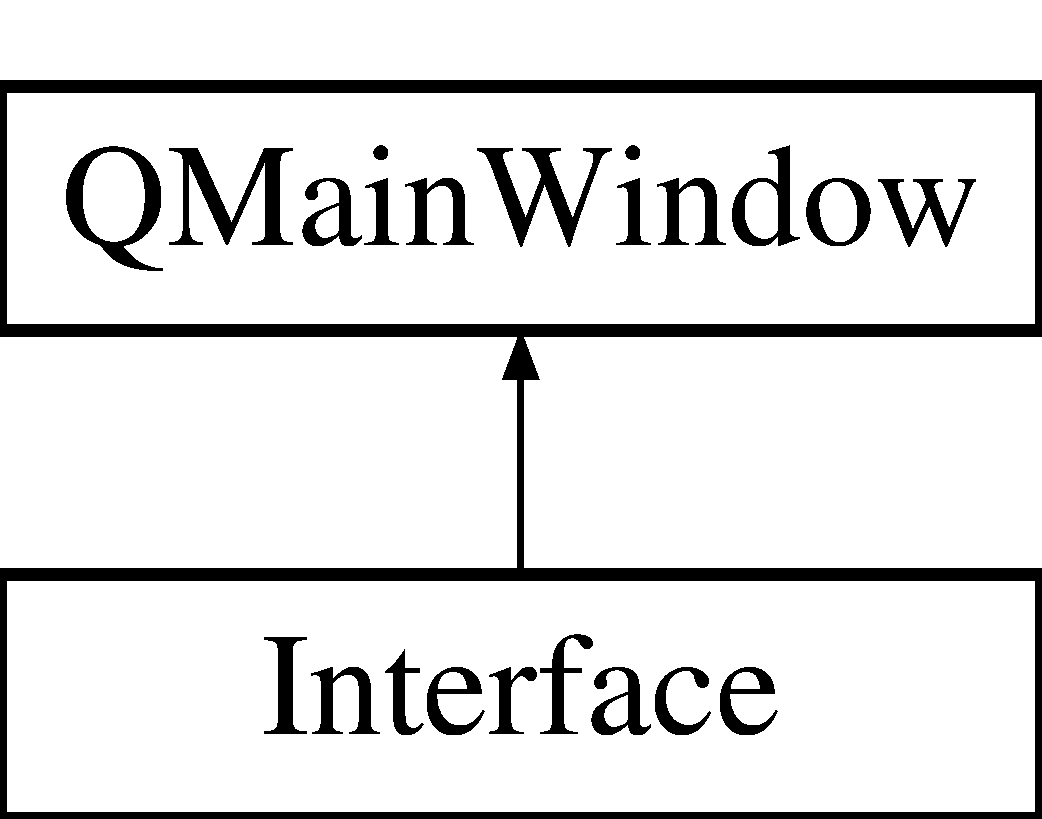
\includegraphics[height=2.000000cm]{class_interface}
\end{center}
\end{figure}
\subsection*{Public Member Functions}
\begin{DoxyCompactItemize}
\item 
\hyperlink{class_interface_a4406d74c75bdfe150bf72be1f1cda8b1}{Interface} ()
\item 
void \hyperlink{class_interface_ab16225b70e5b896ce72ff1f635f4ea80}{creer\+Menu} ()
\item 
void \hyperlink{class_interface_a6e75d088bb17b45927e717cfa02efb46}{creer\+Action\+Menu} ()
\item 
Q\+List$<$ Q\+Table\+Widget\+Item $\ast$ $>$ \hyperlink{class_interface_ad79d4272b59a608ae0c0b48692bdc0fc}{get\+Cellules\+Ligne} ()
\end{DoxyCompactItemize}
\subsection*{Private Slots}
\begin{DoxyCompactItemize}
\item 
void \hyperlink{class_interface_adba89efb181d1e4bc73b1fcaf19da136}{quitter} ()
\item 
void \hyperlink{class_interface_aa1740b524bd3d5a616c3da169b21bbe2}{a\+Propos} ()
\item 
void \hyperlink{class_interface_a2453496cddd1a8f8935c4cee547535b8}{gerer\+Projet} ()
\item 
void \hyperlink{class_interface_a7e65fe818b99979831ea4aea34ce1222}{gerer\+Event} ()
\end{DoxyCompactItemize}
\subsection*{Private Attributes}
\begin{DoxyCompactItemize}
\item 
Q\+Menu $\ast$ \hyperlink{class_interface_a5c22d42f0a82b546269f2265dc4020bf}{options}
\item 
Q\+Menu $\ast$ \hyperlink{class_interface_a8e1bd8a8cfb02dd361ece990addd7515}{aide}
\item 
Q\+Action $\ast$ \hyperlink{class_interface_af2d5dd8a8ec08aca6ef98b14657b2d03}{quitte}
\item 
Q\+Action $\ast$ \hyperlink{class_interface_a2282b9ebbfc4d6b78aff0c4f09edf3ef}{propos}
\item 
Q\+Date\+Edit $\ast$ \hyperlink{class_interface_ac4ca6cf95990077c3c695f54b9340d46}{semaine}
\item 
Q\+Date $\ast$ \hyperlink{class_interface_a25db9c3292f0f8d545d0241f11a59293}{jour\+Courant}
\item 
Q\+Date $\ast$ \hyperlink{class_interface_aa5946e70fad2d32fd4dc55c88bd440e5}{boucle\+Jour}
\item 
Q\+Date $\ast$ \hyperlink{class_interface_afa9df6cf4b8edcdea7e9c31e97c1ab3e}{date\+Courante}
\item 
Q\+Label $\ast$ \hyperlink{class_interface_a0b7d1dff057048c33ff74e0eb8919378}{calendar}
\item 
Q\+V\+Box\+Layout $\ast$ \hyperlink{class_interface_a4d03301a342f9024c1e39009f127a5ec}{layout}
\item 
Q\+H\+Box\+Layout $\ast$ \hyperlink{class_interface_aeb8ae11dbb700b6a19c303a39f80999c}{layout1}
\item 
Q\+Grid\+Layout $\ast$ \hyperlink{class_interface_a99dba2dd8a820785420c7b16677b18a6}{layout2}
\item 
Q\+Grid\+Layout $\ast$ \hyperlink{class_interface_a296d3fd708454c14456b50c56d3f87c4}{layout3}
\item 
Q\+V\+Box\+Layout $\ast$ \hyperlink{class_interface_a723b35155d78820333a349c15f66c4e9}{layout4}
\item 
Q\+V\+Box\+Layout $\ast$ \hyperlink{class_interface_ab996ff872c831e183bace04cc136bb49}{layout5}
\item 
Q\+Table\+Widget $\ast$ \hyperlink{class_interface_add370ece6c97151da99ebab84362c6a1}{table}
\item 
Q\+Calendar\+Widget $\ast$ \hyperlink{class_interface_a53a4b3fb1f0885aea0395658a4b36022}{cal}
\item 
Q\+Group\+Box $\ast$ \hyperlink{class_interface_a2f0340a091c08fb4d6c3357fbd156d21}{menu\+Cote}
\item 
Q\+Push\+Button $\ast$ \hyperlink{class_interface_aa11e7c29121814ee23bafd43ab68b534}{gprojet}
\item 
Q\+Push\+Button $\ast$ \hyperlink{class_interface_a5ad660e0308903af33f1e40daa239010}{gevt}
\item 
Q\+Vector$<$ \hyperlink{class_programmation}{Programmation} $\ast$ $>$ \hyperlink{class_interface_a8c9a2e9fb9a19f879383fb160430c1b6}{prog}
\end{DoxyCompactItemize}


\subsection{Constructor \& Destructor Documentation}
\hypertarget{class_interface_a4406d74c75bdfe150bf72be1f1cda8b1}{}\index{Interface@{Interface}!Interface@{Interface}}
\index{Interface@{Interface}!Interface@{Interface}}
\subsubsection[{Interface}]{\setlength{\rightskip}{0pt plus 5cm}Interface\+::\+Interface (
\begin{DoxyParamCaption}
{}
\end{DoxyParamCaption}
)\hspace{0.3cm}{\ttfamily [explicit]}}\label{class_interface_a4406d74c75bdfe150bf72be1f1cda8b1}


\subsection{Member Function Documentation}
\hypertarget{class_interface_aa1740b524bd3d5a616c3da169b21bbe2}{}\index{Interface@{Interface}!a\+Propos@{a\+Propos}}
\index{a\+Propos@{a\+Propos}!Interface@{Interface}}
\subsubsection[{a\+Propos}]{\setlength{\rightskip}{0pt plus 5cm}void Interface\+::a\+Propos (
\begin{DoxyParamCaption}
{}
\end{DoxyParamCaption}
)\hspace{0.3cm}{\ttfamily [private]}, {\ttfamily [slot]}}\label{class_interface_aa1740b524bd3d5a616c3da169b21bbe2}
\hypertarget{class_interface_a6e75d088bb17b45927e717cfa02efb46}{}\index{Interface@{Interface}!creer\+Action\+Menu@{creer\+Action\+Menu}}
\index{creer\+Action\+Menu@{creer\+Action\+Menu}!Interface@{Interface}}
\subsubsection[{creer\+Action\+Menu}]{\setlength{\rightskip}{0pt plus 5cm}void Interface\+::creer\+Action\+Menu (
\begin{DoxyParamCaption}
{}
\end{DoxyParamCaption}
)}\label{class_interface_a6e75d088bb17b45927e717cfa02efb46}
\hypertarget{class_interface_ab16225b70e5b896ce72ff1f635f4ea80}{}\index{Interface@{Interface}!creer\+Menu@{creer\+Menu}}
\index{creer\+Menu@{creer\+Menu}!Interface@{Interface}}
\subsubsection[{creer\+Menu}]{\setlength{\rightskip}{0pt plus 5cm}void Interface\+::creer\+Menu (
\begin{DoxyParamCaption}
{}
\end{DoxyParamCaption}
)}\label{class_interface_ab16225b70e5b896ce72ff1f635f4ea80}
\hypertarget{class_interface_a7e65fe818b99979831ea4aea34ce1222}{}\index{Interface@{Interface}!gerer\+Event@{gerer\+Event}}
\index{gerer\+Event@{gerer\+Event}!Interface@{Interface}}
\subsubsection[{gerer\+Event}]{\setlength{\rightskip}{0pt plus 5cm}void Interface\+::gerer\+Event (
\begin{DoxyParamCaption}
{}
\end{DoxyParamCaption}
)\hspace{0.3cm}{\ttfamily [private]}, {\ttfamily [slot]}}\label{class_interface_a7e65fe818b99979831ea4aea34ce1222}
\hypertarget{class_interface_a2453496cddd1a8f8935c4cee547535b8}{}\index{Interface@{Interface}!gerer\+Projet@{gerer\+Projet}}
\index{gerer\+Projet@{gerer\+Projet}!Interface@{Interface}}
\subsubsection[{gerer\+Projet}]{\setlength{\rightskip}{0pt plus 5cm}void Interface\+::gerer\+Projet (
\begin{DoxyParamCaption}
{}
\end{DoxyParamCaption}
)\hspace{0.3cm}{\ttfamily [private]}, {\ttfamily [slot]}}\label{class_interface_a2453496cddd1a8f8935c4cee547535b8}
\hypertarget{class_interface_ad79d4272b59a608ae0c0b48692bdc0fc}{}\index{Interface@{Interface}!get\+Cellules\+Ligne@{get\+Cellules\+Ligne}}
\index{get\+Cellules\+Ligne@{get\+Cellules\+Ligne}!Interface@{Interface}}
\subsubsection[{get\+Cellules\+Ligne}]{\setlength{\rightskip}{0pt plus 5cm}Q\+List$<$ Q\+Table\+Widget\+Item $\ast$ $>$ Interface\+::get\+Cellules\+Ligne (
\begin{DoxyParamCaption}
{}
\end{DoxyParamCaption}
)}\label{class_interface_ad79d4272b59a608ae0c0b48692bdc0fc}
\hypertarget{class_interface_adba89efb181d1e4bc73b1fcaf19da136}{}\index{Interface@{Interface}!quitter@{quitter}}
\index{quitter@{quitter}!Interface@{Interface}}
\subsubsection[{quitter}]{\setlength{\rightskip}{0pt plus 5cm}void Interface\+::quitter (
\begin{DoxyParamCaption}
{}
\end{DoxyParamCaption}
)\hspace{0.3cm}{\ttfamily [private]}, {\ttfamily [slot]}}\label{class_interface_adba89efb181d1e4bc73b1fcaf19da136}


\subsection{Member Data Documentation}
\hypertarget{class_interface_a8e1bd8a8cfb02dd361ece990addd7515}{}\index{Interface@{Interface}!aide@{aide}}
\index{aide@{aide}!Interface@{Interface}}
\subsubsection[{aide}]{\setlength{\rightskip}{0pt plus 5cm}Q\+Menu$\ast$ Interface\+::aide\hspace{0.3cm}{\ttfamily [private]}}\label{class_interface_a8e1bd8a8cfb02dd361ece990addd7515}
\hypertarget{class_interface_aa5946e70fad2d32fd4dc55c88bd440e5}{}\index{Interface@{Interface}!boucle\+Jour@{boucle\+Jour}}
\index{boucle\+Jour@{boucle\+Jour}!Interface@{Interface}}
\subsubsection[{boucle\+Jour}]{\setlength{\rightskip}{0pt plus 5cm}Q\+Date$\ast$ Interface\+::boucle\+Jour\hspace{0.3cm}{\ttfamily [private]}}\label{class_interface_aa5946e70fad2d32fd4dc55c88bd440e5}
\hypertarget{class_interface_a53a4b3fb1f0885aea0395658a4b36022}{}\index{Interface@{Interface}!cal@{cal}}
\index{cal@{cal}!Interface@{Interface}}
\subsubsection[{cal}]{\setlength{\rightskip}{0pt plus 5cm}Q\+Calendar\+Widget$\ast$ Interface\+::cal\hspace{0.3cm}{\ttfamily [private]}}\label{class_interface_a53a4b3fb1f0885aea0395658a4b36022}
\hypertarget{class_interface_a0b7d1dff057048c33ff74e0eb8919378}{}\index{Interface@{Interface}!calendar@{calendar}}
\index{calendar@{calendar}!Interface@{Interface}}
\subsubsection[{calendar}]{\setlength{\rightskip}{0pt plus 5cm}Q\+Label$\ast$ Interface\+::calendar\hspace{0.3cm}{\ttfamily [private]}}\label{class_interface_a0b7d1dff057048c33ff74e0eb8919378}
\hypertarget{class_interface_afa9df6cf4b8edcdea7e9c31e97c1ab3e}{}\index{Interface@{Interface}!date\+Courante@{date\+Courante}}
\index{date\+Courante@{date\+Courante}!Interface@{Interface}}
\subsubsection[{date\+Courante}]{\setlength{\rightskip}{0pt plus 5cm}Q\+Date$\ast$ Interface\+::date\+Courante\hspace{0.3cm}{\ttfamily [private]}}\label{class_interface_afa9df6cf4b8edcdea7e9c31e97c1ab3e}
\hypertarget{class_interface_a5ad660e0308903af33f1e40daa239010}{}\index{Interface@{Interface}!gevt@{gevt}}
\index{gevt@{gevt}!Interface@{Interface}}
\subsubsection[{gevt}]{\setlength{\rightskip}{0pt plus 5cm}Q\+Push\+Button$\ast$ Interface\+::gevt\hspace{0.3cm}{\ttfamily [private]}}\label{class_interface_a5ad660e0308903af33f1e40daa239010}
\hypertarget{class_interface_aa11e7c29121814ee23bafd43ab68b534}{}\index{Interface@{Interface}!gprojet@{gprojet}}
\index{gprojet@{gprojet}!Interface@{Interface}}
\subsubsection[{gprojet}]{\setlength{\rightskip}{0pt plus 5cm}Q\+Push\+Button$\ast$ Interface\+::gprojet\hspace{0.3cm}{\ttfamily [private]}}\label{class_interface_aa11e7c29121814ee23bafd43ab68b534}
\hypertarget{class_interface_a25db9c3292f0f8d545d0241f11a59293}{}\index{Interface@{Interface}!jour\+Courant@{jour\+Courant}}
\index{jour\+Courant@{jour\+Courant}!Interface@{Interface}}
\subsubsection[{jour\+Courant}]{\setlength{\rightskip}{0pt plus 5cm}Q\+Date$\ast$ Interface\+::jour\+Courant\hspace{0.3cm}{\ttfamily [private]}}\label{class_interface_a25db9c3292f0f8d545d0241f11a59293}
\hypertarget{class_interface_a4d03301a342f9024c1e39009f127a5ec}{}\index{Interface@{Interface}!layout@{layout}}
\index{layout@{layout}!Interface@{Interface}}
\subsubsection[{layout}]{\setlength{\rightskip}{0pt plus 5cm}Q\+V\+Box\+Layout$\ast$ Interface\+::layout\hspace{0.3cm}{\ttfamily [private]}}\label{class_interface_a4d03301a342f9024c1e39009f127a5ec}
\hypertarget{class_interface_aeb8ae11dbb700b6a19c303a39f80999c}{}\index{Interface@{Interface}!layout1@{layout1}}
\index{layout1@{layout1}!Interface@{Interface}}
\subsubsection[{layout1}]{\setlength{\rightskip}{0pt plus 5cm}Q\+H\+Box\+Layout$\ast$ Interface\+::layout1\hspace{0.3cm}{\ttfamily [private]}}\label{class_interface_aeb8ae11dbb700b6a19c303a39f80999c}
\hypertarget{class_interface_a99dba2dd8a820785420c7b16677b18a6}{}\index{Interface@{Interface}!layout2@{layout2}}
\index{layout2@{layout2}!Interface@{Interface}}
\subsubsection[{layout2}]{\setlength{\rightskip}{0pt plus 5cm}Q\+Grid\+Layout$\ast$ Interface\+::layout2\hspace{0.3cm}{\ttfamily [private]}}\label{class_interface_a99dba2dd8a820785420c7b16677b18a6}
\hypertarget{class_interface_a296d3fd708454c14456b50c56d3f87c4}{}\index{Interface@{Interface}!layout3@{layout3}}
\index{layout3@{layout3}!Interface@{Interface}}
\subsubsection[{layout3}]{\setlength{\rightskip}{0pt plus 5cm}Q\+Grid\+Layout$\ast$ Interface\+::layout3\hspace{0.3cm}{\ttfamily [private]}}\label{class_interface_a296d3fd708454c14456b50c56d3f87c4}
\hypertarget{class_interface_a723b35155d78820333a349c15f66c4e9}{}\index{Interface@{Interface}!layout4@{layout4}}
\index{layout4@{layout4}!Interface@{Interface}}
\subsubsection[{layout4}]{\setlength{\rightskip}{0pt plus 5cm}Q\+V\+Box\+Layout$\ast$ Interface\+::layout4\hspace{0.3cm}{\ttfamily [private]}}\label{class_interface_a723b35155d78820333a349c15f66c4e9}
\hypertarget{class_interface_ab996ff872c831e183bace04cc136bb49}{}\index{Interface@{Interface}!layout5@{layout5}}
\index{layout5@{layout5}!Interface@{Interface}}
\subsubsection[{layout5}]{\setlength{\rightskip}{0pt plus 5cm}Q\+V\+Box\+Layout$\ast$ Interface\+::layout5\hspace{0.3cm}{\ttfamily [private]}}\label{class_interface_ab996ff872c831e183bace04cc136bb49}
\hypertarget{class_interface_a2f0340a091c08fb4d6c3357fbd156d21}{}\index{Interface@{Interface}!menu\+Cote@{menu\+Cote}}
\index{menu\+Cote@{menu\+Cote}!Interface@{Interface}}
\subsubsection[{menu\+Cote}]{\setlength{\rightskip}{0pt plus 5cm}Q\+Group\+Box$\ast$ Interface\+::menu\+Cote\hspace{0.3cm}{\ttfamily [private]}}\label{class_interface_a2f0340a091c08fb4d6c3357fbd156d21}
\hypertarget{class_interface_a5c22d42f0a82b546269f2265dc4020bf}{}\index{Interface@{Interface}!options@{options}}
\index{options@{options}!Interface@{Interface}}
\subsubsection[{options}]{\setlength{\rightskip}{0pt plus 5cm}Q\+Menu$\ast$ Interface\+::options\hspace{0.3cm}{\ttfamily [private]}}\label{class_interface_a5c22d42f0a82b546269f2265dc4020bf}
\hypertarget{class_interface_a8c9a2e9fb9a19f879383fb160430c1b6}{}\index{Interface@{Interface}!prog@{prog}}
\index{prog@{prog}!Interface@{Interface}}
\subsubsection[{prog}]{\setlength{\rightskip}{0pt plus 5cm}Q\+Vector$<${\bf Programmation}$\ast$$>$ Interface\+::prog\hspace{0.3cm}{\ttfamily [private]}}\label{class_interface_a8c9a2e9fb9a19f879383fb160430c1b6}
\hypertarget{class_interface_a2282b9ebbfc4d6b78aff0c4f09edf3ef}{}\index{Interface@{Interface}!propos@{propos}}
\index{propos@{propos}!Interface@{Interface}}
\subsubsection[{propos}]{\setlength{\rightskip}{0pt plus 5cm}Q\+Action$\ast$ Interface\+::propos\hspace{0.3cm}{\ttfamily [private]}}\label{class_interface_a2282b9ebbfc4d6b78aff0c4f09edf3ef}
\hypertarget{class_interface_af2d5dd8a8ec08aca6ef98b14657b2d03}{}\index{Interface@{Interface}!quitte@{quitte}}
\index{quitte@{quitte}!Interface@{Interface}}
\subsubsection[{quitte}]{\setlength{\rightskip}{0pt plus 5cm}Q\+Action$\ast$ Interface\+::quitte\hspace{0.3cm}{\ttfamily [private]}}\label{class_interface_af2d5dd8a8ec08aca6ef98b14657b2d03}
\hypertarget{class_interface_ac4ca6cf95990077c3c695f54b9340d46}{}\index{Interface@{Interface}!semaine@{semaine}}
\index{semaine@{semaine}!Interface@{Interface}}
\subsubsection[{semaine}]{\setlength{\rightskip}{0pt plus 5cm}Q\+Date\+Edit$\ast$ Interface\+::semaine\hspace{0.3cm}{\ttfamily [private]}}\label{class_interface_ac4ca6cf95990077c3c695f54b9340d46}
\hypertarget{class_interface_add370ece6c97151da99ebab84362c6a1}{}\index{Interface@{Interface}!table@{table}}
\index{table@{table}!Interface@{Interface}}
\subsubsection[{table}]{\setlength{\rightskip}{0pt plus 5cm}Q\+Table\+Widget$\ast$ Interface\+::table\hspace{0.3cm}{\ttfamily [private]}}\label{class_interface_add370ece6c97151da99ebab84362c6a1}


The documentation for this class was generated from the following files\+:\begin{DoxyCompactItemize}
\item 
projet/\hyperlink{interface_8h}{interface.\+h}\item 
projet/\hyperlink{interface_8cpp}{interface.\+cpp}\end{DoxyCompactItemize}

\hypertarget{class_liste_projets}{}\section{Liste\+Projets Class Reference}
\label{class_liste_projets}\index{Liste\+Projets@{Liste\+Projets}}


{\ttfamily \#include $<$listeprojets.\+h$>$}

Inheritance diagram for Liste\+Projets\+:\begin{figure}[H]
\begin{center}
\leavevmode
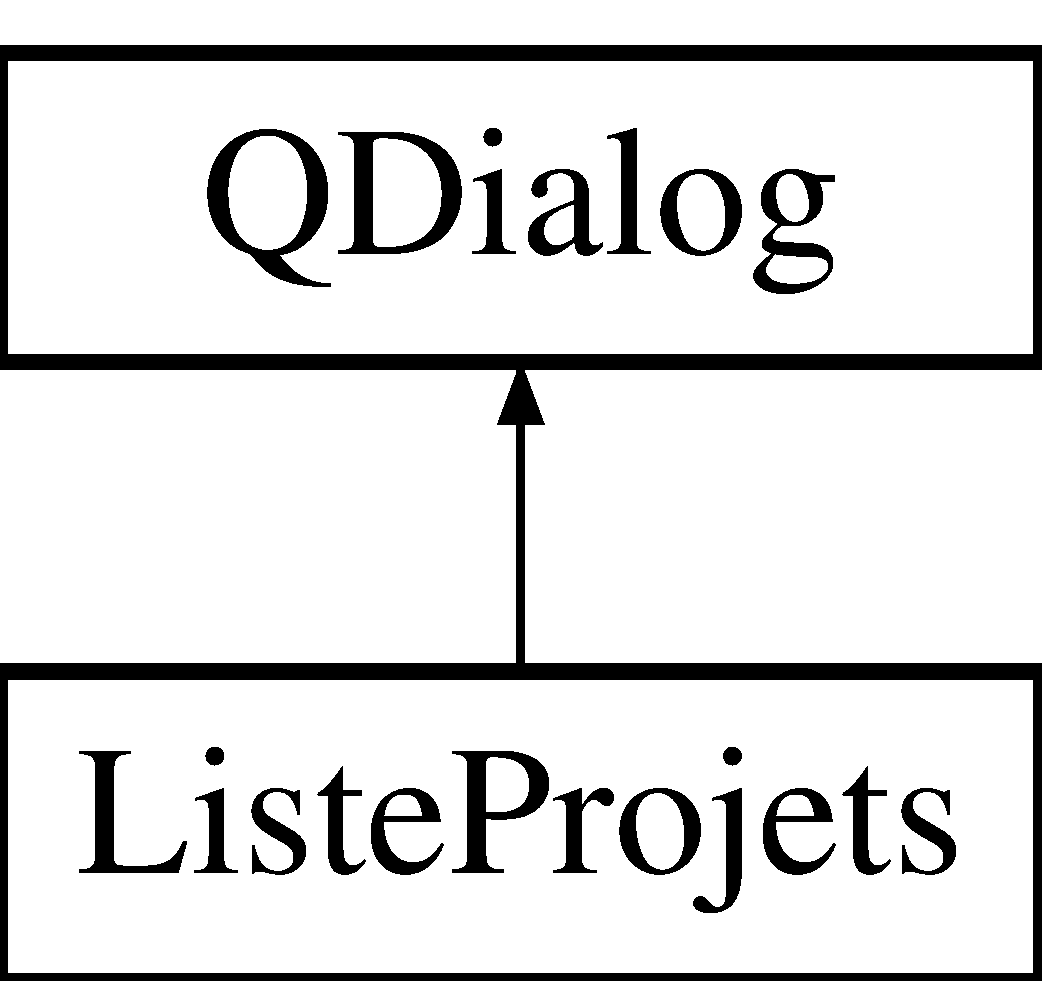
\includegraphics[height=2.000000cm]{class_liste_projets}
\end{center}
\end{figure}
\subsection*{Signals}
\begin{DoxyCompactItemize}
\item 
void \hyperlink{class_liste_projets_ac5a81b7b05afd8678cf82899e1504266}{clicked} (int)
\end{DoxyCompactItemize}
\subsection*{Public Member Functions}
\begin{DoxyCompactItemize}
\item 
\hyperlink{class_liste_projets_a069a958b17e8a03352716875bcd7fe80}{Liste\+Projets} (Q\+Widget $\ast$parent=0)
\end{DoxyCompactItemize}
\subsection*{Public Attributes}
\begin{DoxyCompactItemize}
\item 
Q\+V\+Box\+Layout $\ast$ \hyperlink{class_liste_projets_a5e745a69ba95eeae29269022a08becc4}{layout}
\item 
Q\+Push\+Button $\ast$ \hyperlink{class_liste_projets_ad38087a7e6e7f418ced454ad24f3db72}{add\+Prj}
\item 
Q\+Push\+Button $\ast$ \hyperlink{class_liste_projets_a0c34df5d18031dd6830eac4e7c3ee9ac}{bouton}
\item 
Q\+Vector$<$ \hyperlink{class_projet}{Projet} $\ast$ $>$ \hyperlink{class_liste_projets_a675688a1c030d0555daf8d968eaae50c}{prj}
\end{DoxyCompactItemize}
\subsection*{Private Slots}
\begin{DoxyCompactItemize}
\item 
void \hyperlink{class_liste_projets_aa24f013af28d699a6f78fe4142300228}{afficher\+Projet} (int i)
\item 
void \hyperlink{class_liste_projets_a7e51fd74bc104e3c73aa4f53a10853c5}{ajouter\+Projet} ()
\end{DoxyCompactItemize}
\subsection*{Private Attributes}
\begin{DoxyCompactItemize}
\item 
Q\+Signal\+Mapper $\ast$ \hyperlink{class_liste_projets_ab155bcfe455d8951c5ba057e118d10c9}{sm}
\end{DoxyCompactItemize}


\subsection{Constructor \& Destructor Documentation}
\hypertarget{class_liste_projets_a069a958b17e8a03352716875bcd7fe80}{}\index{Liste\+Projets@{Liste\+Projets}!Liste\+Projets@{Liste\+Projets}}
\index{Liste\+Projets@{Liste\+Projets}!Liste\+Projets@{Liste\+Projets}}
\subsubsection[{Liste\+Projets}]{\setlength{\rightskip}{0pt plus 5cm}Liste\+Projets\+::\+Liste\+Projets (
\begin{DoxyParamCaption}
\item[{Q\+Widget $\ast$}]{parent = {\ttfamily 0}}
\end{DoxyParamCaption}
)\hspace{0.3cm}{\ttfamily [explicit]}}\label{class_liste_projets_a069a958b17e8a03352716875bcd7fe80}


\subsection{Member Function Documentation}
\hypertarget{class_liste_projets_aa24f013af28d699a6f78fe4142300228}{}\index{Liste\+Projets@{Liste\+Projets}!afficher\+Projet@{afficher\+Projet}}
\index{afficher\+Projet@{afficher\+Projet}!Liste\+Projets@{Liste\+Projets}}
\subsubsection[{afficher\+Projet}]{\setlength{\rightskip}{0pt plus 5cm}void Liste\+Projets\+::afficher\+Projet (
\begin{DoxyParamCaption}
\item[{int}]{i}
\end{DoxyParamCaption}
)\hspace{0.3cm}{\ttfamily [private]}, {\ttfamily [slot]}}\label{class_liste_projets_aa24f013af28d699a6f78fe4142300228}
\hypertarget{class_liste_projets_a7e51fd74bc104e3c73aa4f53a10853c5}{}\index{Liste\+Projets@{Liste\+Projets}!ajouter\+Projet@{ajouter\+Projet}}
\index{ajouter\+Projet@{ajouter\+Projet}!Liste\+Projets@{Liste\+Projets}}
\subsubsection[{ajouter\+Projet}]{\setlength{\rightskip}{0pt plus 5cm}void Liste\+Projets\+::ajouter\+Projet (
\begin{DoxyParamCaption}
{}
\end{DoxyParamCaption}
)\hspace{0.3cm}{\ttfamily [private]}, {\ttfamily [slot]}}\label{class_liste_projets_a7e51fd74bc104e3c73aa4f53a10853c5}
\hypertarget{class_liste_projets_ac5a81b7b05afd8678cf82899e1504266}{}\index{Liste\+Projets@{Liste\+Projets}!clicked@{clicked}}
\index{clicked@{clicked}!Liste\+Projets@{Liste\+Projets}}
\subsubsection[{clicked}]{\setlength{\rightskip}{0pt plus 5cm}void Liste\+Projets\+::clicked (
\begin{DoxyParamCaption}
\item[{int}]{}
\end{DoxyParamCaption}
)\hspace{0.3cm}{\ttfamily [signal]}}\label{class_liste_projets_ac5a81b7b05afd8678cf82899e1504266}


\subsection{Member Data Documentation}
\hypertarget{class_liste_projets_ad38087a7e6e7f418ced454ad24f3db72}{}\index{Liste\+Projets@{Liste\+Projets}!add\+Prj@{add\+Prj}}
\index{add\+Prj@{add\+Prj}!Liste\+Projets@{Liste\+Projets}}
\subsubsection[{add\+Prj}]{\setlength{\rightskip}{0pt plus 5cm}Q\+Push\+Button$\ast$ Liste\+Projets\+::add\+Prj}\label{class_liste_projets_ad38087a7e6e7f418ced454ad24f3db72}
\hypertarget{class_liste_projets_a0c34df5d18031dd6830eac4e7c3ee9ac}{}\index{Liste\+Projets@{Liste\+Projets}!bouton@{bouton}}
\index{bouton@{bouton}!Liste\+Projets@{Liste\+Projets}}
\subsubsection[{bouton}]{\setlength{\rightskip}{0pt plus 5cm}Q\+Push\+Button$\ast$ Liste\+Projets\+::bouton}\label{class_liste_projets_a0c34df5d18031dd6830eac4e7c3ee9ac}
\hypertarget{class_liste_projets_a5e745a69ba95eeae29269022a08becc4}{}\index{Liste\+Projets@{Liste\+Projets}!layout@{layout}}
\index{layout@{layout}!Liste\+Projets@{Liste\+Projets}}
\subsubsection[{layout}]{\setlength{\rightskip}{0pt plus 5cm}Q\+V\+Box\+Layout$\ast$ Liste\+Projets\+::layout}\label{class_liste_projets_a5e745a69ba95eeae29269022a08becc4}
\hypertarget{class_liste_projets_a675688a1c030d0555daf8d968eaae50c}{}\index{Liste\+Projets@{Liste\+Projets}!prj@{prj}}
\index{prj@{prj}!Liste\+Projets@{Liste\+Projets}}
\subsubsection[{prj}]{\setlength{\rightskip}{0pt plus 5cm}Q\+Vector$<${\bf Projet}$\ast$$>$ Liste\+Projets\+::prj}\label{class_liste_projets_a675688a1c030d0555daf8d968eaae50c}
\hypertarget{class_liste_projets_ab155bcfe455d8951c5ba057e118d10c9}{}\index{Liste\+Projets@{Liste\+Projets}!sm@{sm}}
\index{sm@{sm}!Liste\+Projets@{Liste\+Projets}}
\subsubsection[{sm}]{\setlength{\rightskip}{0pt plus 5cm}Q\+Signal\+Mapper$\ast$ Liste\+Projets\+::sm\hspace{0.3cm}{\ttfamily [private]}}\label{class_liste_projets_ab155bcfe455d8951c5ba057e118d10c9}


The documentation for this class was generated from the following files\+:\begin{DoxyCompactItemize}
\item 
projet/\hyperlink{listeprojets_8h}{listeprojets.\+h}\item 
projet/\hyperlink{listeprojets_8cpp}{listeprojets.\+cpp}\end{DoxyCompactItemize}

\hypertarget{class_main_window}{}\section{Référence de la classe Main\+Window}
\label{class_main_window}\index{Main\+Window@{Main\+Window}}


{\ttfamily \#include $<$mainwindow.\+h$>$}

Graphe d\textquotesingle{}héritage de Main\+Window\+:\begin{figure}[H]
\begin{center}
\leavevmode
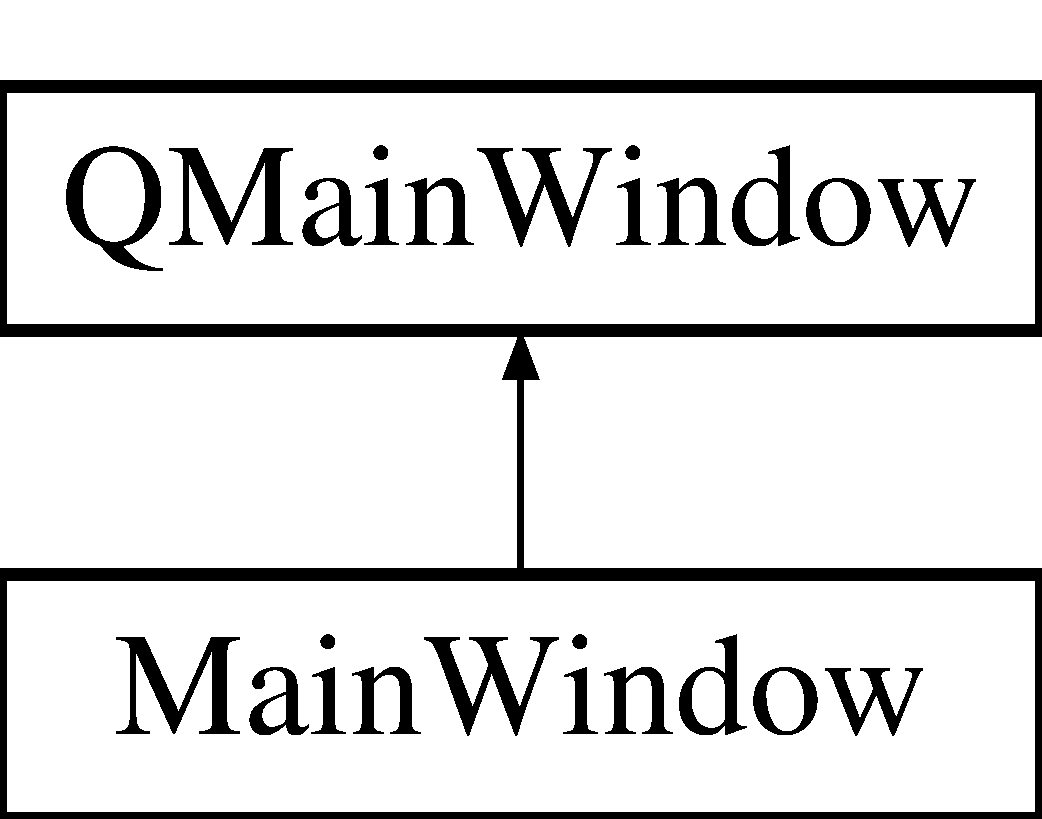
\includegraphics[height=2.000000cm]{class_main_window}
\end{center}
\end{figure}
\subsection*{Fonctions membres publiques}
\begin{DoxyCompactItemize}
\item 
\hyperlink{class_main_window_a8b244be8b7b7db1b08de2a2acb9409db}{Main\+Window} (Q\+Widget $\ast$parent=0)
\item 
\hyperlink{class_main_window_ae98d00a93bc118200eeef9f9bba1dba7}{$\sim$\+Main\+Window} ()
\end{DoxyCompactItemize}
\subsection*{Attributs privés}
\begin{DoxyCompactItemize}
\item 
Ui\+::\+Main\+Window $\ast$ \hyperlink{class_main_window_a35466a70ed47252a0191168126a352a5}{ui}
\end{DoxyCompactItemize}


\subsection{Documentation des constructeurs et destructeur}
\hypertarget{class_main_window_a8b244be8b7b7db1b08de2a2acb9409db}{}\index{Main\+Window@{Main\+Window}!Main\+Window@{Main\+Window}}
\index{Main\+Window@{Main\+Window}!Main\+Window@{Main\+Window}}
\subsubsection[{Main\+Window}]{\setlength{\rightskip}{0pt plus 5cm}Main\+Window\+::\+Main\+Window (
\begin{DoxyParamCaption}
\item[{Q\+Widget $\ast$}]{parent = {\ttfamily 0}}
\end{DoxyParamCaption}
)\hspace{0.3cm}{\ttfamily [explicit]}}\label{class_main_window_a8b244be8b7b7db1b08de2a2acb9409db}
\hypertarget{class_main_window_ae98d00a93bc118200eeef9f9bba1dba7}{}\index{Main\+Window@{Main\+Window}!````~Main\+Window@{$\sim$\+Main\+Window}}
\index{````~Main\+Window@{$\sim$\+Main\+Window}!Main\+Window@{Main\+Window}}
\subsubsection[{$\sim$\+Main\+Window}]{\setlength{\rightskip}{0pt plus 5cm}Main\+Window\+::$\sim$\+Main\+Window (
\begin{DoxyParamCaption}
{}
\end{DoxyParamCaption}
)}\label{class_main_window_ae98d00a93bc118200eeef9f9bba1dba7}


\subsection{Documentation des données membres}
\hypertarget{class_main_window_a35466a70ed47252a0191168126a352a5}{}\index{Main\+Window@{Main\+Window}!ui@{ui}}
\index{ui@{ui}!Main\+Window@{Main\+Window}}
\subsubsection[{ui}]{\setlength{\rightskip}{0pt plus 5cm}Ui\+::\+Main\+Window$\ast$ Main\+Window\+::ui\hspace{0.3cm}{\ttfamily [private]}}\label{class_main_window_a35466a70ed47252a0191168126a352a5}


La documentation de cette classe a été générée à partir des fichiers suivants \+:\begin{DoxyCompactItemize}
\item 
\hyperlink{mainwindow_8h}{mainwindow.\+h}\item 
\hyperlink{mainwindow_8cpp}{mainwindow.\+cpp}\end{DoxyCompactItemize}

\hypertarget{class_programmation}{}\section{Programmation Class Reference}
\label{class_programmation}\index{Programmation@{Programmation}}


{\ttfamily \#include $<$programmation.\+h$>$}

Inheritance diagram for Programmation\+:\begin{figure}[H]
\begin{center}
\leavevmode
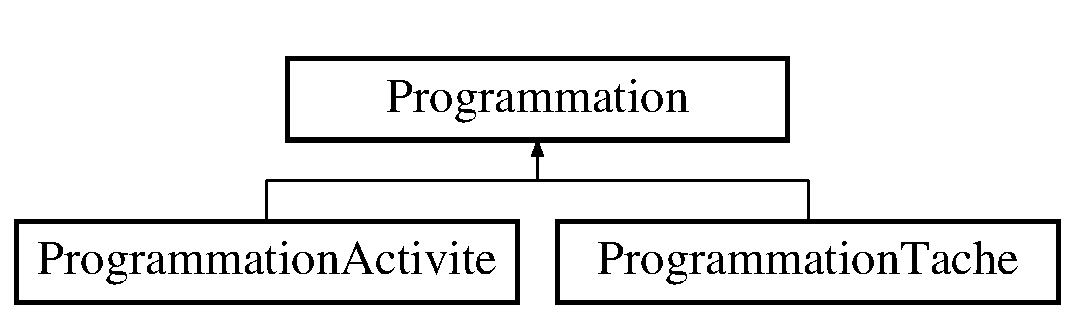
\includegraphics[height=2.000000cm]{class_programmation}
\end{center}
\end{figure}
\subsection*{Public Member Functions}
\begin{DoxyCompactItemize}
\item 
Q\+String \hyperlink{class_programmation_a37380f79c4235bfedcbab7c2b9c5de5c}{get\+Identifiant} () const 
\item 
Q\+Date \hyperlink{class_programmation_abd1632dfa907a6bf2a84bfdbc3bef38f}{get\+Date} () const 
\item 
int \hyperlink{class_programmation_a927a5f9c0c752d33d12eb100b9315055}{get\+Heure\+Debut} () const 
\item 
int \hyperlink{class_programmation_a8ebc1580f9e4a3a3317d4a5535e28d8b}{get\+Heure\+Fin} () const 
\end{DoxyCompactItemize}
\subsection*{Protected Member Functions}
\begin{DoxyCompactItemize}
\item 
\hyperlink{class_programmation_a73e7d51291b37140ffb7647bfa0d5ff3}{Programmation} (Q\+String id, Q\+Date dat, int hd, int hf)
\item 
virtual \hyperlink{class_programmation_aa477667deb545f10a3f5d32d7a3df590}{$\sim$\+Programmation} ()
\end{DoxyCompactItemize}
\subsection*{Protected Attributes}
\begin{DoxyCompactItemize}
\item 
Q\+String \hyperlink{class_programmation_aea36cbc16a71cead5fed20ce8b7670fc}{identifiant}
\item 
Q\+Date \hyperlink{class_programmation_a993696842e7ec41f37aa9c0e7e383296}{date}
\item 
int \hyperlink{class_programmation_a1456089cb1f36c1f93e8e001a3181add}{heure\+Debut}
\item 
int \hyperlink{class_programmation_a6a807cdfb835c2440834ea04e1ef9d40}{heure\+Fin}
\end{DoxyCompactItemize}
\subsection*{Friends}
\begin{DoxyCompactItemize}
\item 
class \hyperlink{class_programmation_ade7bfcbf8cec66b12064c8ff25993d73}{Programmation\+Manager}
\end{DoxyCompactItemize}


\subsection{Constructor \& Destructor Documentation}
\hypertarget{class_programmation_a73e7d51291b37140ffb7647bfa0d5ff3}{}\index{Programmation@{Programmation}!Programmation@{Programmation}}
\index{Programmation@{Programmation}!Programmation@{Programmation}}
\subsubsection[{Programmation}]{\setlength{\rightskip}{0pt plus 5cm}Programmation\+::\+Programmation (
\begin{DoxyParamCaption}
\item[{Q\+String}]{id, }
\item[{Q\+Date}]{dat, }
\item[{int}]{hd, }
\item[{int}]{hf}
\end{DoxyParamCaption}
)\hspace{0.3cm}{\ttfamily [protected]}}\label{class_programmation_a73e7d51291b37140ffb7647bfa0d5ff3}
\hypertarget{class_programmation_aa477667deb545f10a3f5d32d7a3df590}{}\index{Programmation@{Programmation}!````~Programmation@{$\sim$\+Programmation}}
\index{````~Programmation@{$\sim$\+Programmation}!Programmation@{Programmation}}
\subsubsection[{$\sim$\+Programmation}]{\setlength{\rightskip}{0pt plus 5cm}Programmation\+::$\sim$\+Programmation (
\begin{DoxyParamCaption}
{}
\end{DoxyParamCaption}
)\hspace{0.3cm}{\ttfamily [protected]}, {\ttfamily [virtual]}}\label{class_programmation_aa477667deb545f10a3f5d32d7a3df590}


\subsection{Member Function Documentation}
\hypertarget{class_programmation_abd1632dfa907a6bf2a84bfdbc3bef38f}{}\index{Programmation@{Programmation}!get\+Date@{get\+Date}}
\index{get\+Date@{get\+Date}!Programmation@{Programmation}}
\subsubsection[{get\+Date}]{\setlength{\rightskip}{0pt plus 5cm}Q\+Date Programmation\+::get\+Date (
\begin{DoxyParamCaption}
{}
\end{DoxyParamCaption}
) const\hspace{0.3cm}{\ttfamily [inline]}}\label{class_programmation_abd1632dfa907a6bf2a84bfdbc3bef38f}
\hypertarget{class_programmation_a927a5f9c0c752d33d12eb100b9315055}{}\index{Programmation@{Programmation}!get\+Heure\+Debut@{get\+Heure\+Debut}}
\index{get\+Heure\+Debut@{get\+Heure\+Debut}!Programmation@{Programmation}}
\subsubsection[{get\+Heure\+Debut}]{\setlength{\rightskip}{0pt plus 5cm}int Programmation\+::get\+Heure\+Debut (
\begin{DoxyParamCaption}
{}
\end{DoxyParamCaption}
) const\hspace{0.3cm}{\ttfamily [inline]}}\label{class_programmation_a927a5f9c0c752d33d12eb100b9315055}
\hypertarget{class_programmation_a8ebc1580f9e4a3a3317d4a5535e28d8b}{}\index{Programmation@{Programmation}!get\+Heure\+Fin@{get\+Heure\+Fin}}
\index{get\+Heure\+Fin@{get\+Heure\+Fin}!Programmation@{Programmation}}
\subsubsection[{get\+Heure\+Fin}]{\setlength{\rightskip}{0pt plus 5cm}int Programmation\+::get\+Heure\+Fin (
\begin{DoxyParamCaption}
{}
\end{DoxyParamCaption}
) const\hspace{0.3cm}{\ttfamily [inline]}}\label{class_programmation_a8ebc1580f9e4a3a3317d4a5535e28d8b}
\hypertarget{class_programmation_a37380f79c4235bfedcbab7c2b9c5de5c}{}\index{Programmation@{Programmation}!get\+Identifiant@{get\+Identifiant}}
\index{get\+Identifiant@{get\+Identifiant}!Programmation@{Programmation}}
\subsubsection[{get\+Identifiant}]{\setlength{\rightskip}{0pt plus 5cm}Q\+String Programmation\+::get\+Identifiant (
\begin{DoxyParamCaption}
{}
\end{DoxyParamCaption}
) const\hspace{0.3cm}{\ttfamily [inline]}}\label{class_programmation_a37380f79c4235bfedcbab7c2b9c5de5c}


\subsection{Friends And Related Function Documentation}
\hypertarget{class_programmation_ade7bfcbf8cec66b12064c8ff25993d73}{}\index{Programmation@{Programmation}!Programmation\+Manager@{Programmation\+Manager}}
\index{Programmation\+Manager@{Programmation\+Manager}!Programmation@{Programmation}}
\subsubsection[{Programmation\+Manager}]{\setlength{\rightskip}{0pt plus 5cm}friend class {\bf Programmation\+Manager}\hspace{0.3cm}{\ttfamily [friend]}}\label{class_programmation_ade7bfcbf8cec66b12064c8ff25993d73}


\subsection{Member Data Documentation}
\hypertarget{class_programmation_a993696842e7ec41f37aa9c0e7e383296}{}\index{Programmation@{Programmation}!date@{date}}
\index{date@{date}!Programmation@{Programmation}}
\subsubsection[{date}]{\setlength{\rightskip}{0pt plus 5cm}Q\+Date Programmation\+::date\hspace{0.3cm}{\ttfamily [protected]}}\label{class_programmation_a993696842e7ec41f37aa9c0e7e383296}
\hypertarget{class_programmation_a1456089cb1f36c1f93e8e001a3181add}{}\index{Programmation@{Programmation}!heure\+Debut@{heure\+Debut}}
\index{heure\+Debut@{heure\+Debut}!Programmation@{Programmation}}
\subsubsection[{heure\+Debut}]{\setlength{\rightskip}{0pt plus 5cm}int Programmation\+::heure\+Debut\hspace{0.3cm}{\ttfamily [protected]}}\label{class_programmation_a1456089cb1f36c1f93e8e001a3181add}
\hypertarget{class_programmation_a6a807cdfb835c2440834ea04e1ef9d40}{}\index{Programmation@{Programmation}!heure\+Fin@{heure\+Fin}}
\index{heure\+Fin@{heure\+Fin}!Programmation@{Programmation}}
\subsubsection[{heure\+Fin}]{\setlength{\rightskip}{0pt plus 5cm}int Programmation\+::heure\+Fin\hspace{0.3cm}{\ttfamily [protected]}}\label{class_programmation_a6a807cdfb835c2440834ea04e1ef9d40}
\hypertarget{class_programmation_aea36cbc16a71cead5fed20ce8b7670fc}{}\index{Programmation@{Programmation}!identifiant@{identifiant}}
\index{identifiant@{identifiant}!Programmation@{Programmation}}
\subsubsection[{identifiant}]{\setlength{\rightskip}{0pt plus 5cm}Q\+String Programmation\+::identifiant\hspace{0.3cm}{\ttfamily [protected]}}\label{class_programmation_aea36cbc16a71cead5fed20ce8b7670fc}


The documentation for this class was generated from the following files\+:\begin{DoxyCompactItemize}
\item 
projet/\hyperlink{programmation_8h}{programmation.\+h}\item 
projet/\hyperlink{programmation_8cpp}{programmation.\+cpp}\end{DoxyCompactItemize}

\hypertarget{class_programmation_activite}{}\section{Programmation\+Activite Class Reference}
\label{class_programmation_activite}\index{Programmation\+Activite@{Programmation\+Activite}}


Classe représentant une \hyperlink{class_programmation_activite}{Programmation\+Activite}.  




{\ttfamily \#include $<$programmationactivite.\+h$>$}

Inheritance diagram for Programmation\+Activite\+:\begin{figure}[H]
\begin{center}
\leavevmode
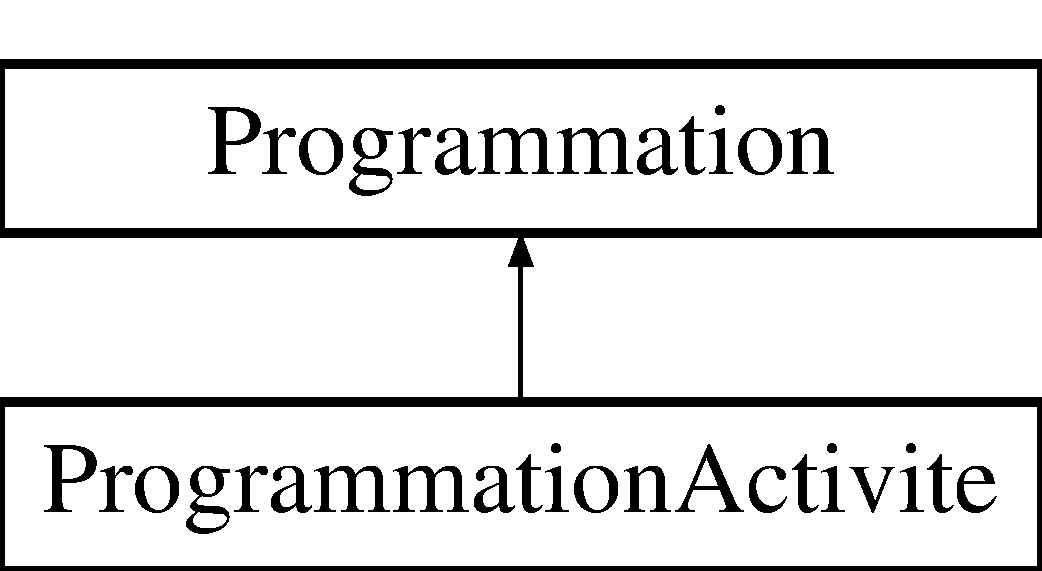
\includegraphics[height=2.000000cm]{class_programmation_activite}
\end{center}
\end{figure}
\subsection*{Public Member Functions}
\begin{DoxyCompactItemize}
\item 
Q\+String \hyperlink{class_programmation_activite_a8a29a5c0e39ad57aaf2ed73c8a004d3c}{get\+Titre} () const 
\item 
Q\+String \hyperlink{class_programmation_activite_a91de19dc76479adeddac07b5a259c026}{get\+Descritpion} () const 
\end{DoxyCompactItemize}
\subsection*{Private Member Functions}
\begin{DoxyCompactItemize}
\item 
\hyperlink{class_programmation_activite_a2492901bfd220779a942fabade7486d1}{Programmation\+Activite} (Q\+String id, Q\+Date dat, int hd, int hf, Q\+String tit, Q\+String desc)
\item 
virtual \hyperlink{class_programmation_activite_acd35d754d36b98a94b5b846378100c33}{$\sim$\+Programmation\+Activite} ()
\end{DoxyCompactItemize}
\subsection*{Private Attributes}
\begin{DoxyCompactItemize}
\item 
Q\+String \hyperlink{class_programmation_activite_aa6f6ff264184635b35615abb4e45ab62}{titre}
\item 
Q\+String \hyperlink{class_programmation_activite_ae2a01c5cfffda9813ae77c1b98c7a52b}{description}
\end{DoxyCompactItemize}
\subsection*{Friends}
\begin{DoxyCompactItemize}
\item 
class \hyperlink{class_programmation_activite_ade7bfcbf8cec66b12064c8ff25993d73}{Programmation\+Manager}
\end{DoxyCompactItemize}
\subsection*{Additional Inherited Members}


\subsection{Detailed Description}
Classe représentant une \hyperlink{class_programmation_activite}{Programmation\+Activite}. 

Une \hyperlink{class_programmation_activite}{Programmation\+Activite} est un événement et donc une \hyperlink{class_programmation}{Programmation}. \hyperlink{class_programmation_activite}{Programmation\+Activite} hérite donc de \hyperlink{class_programmation}{Programmation}. Elle est la programmation d\textquotesingle{}une activité donnée. 

\subsection{Constructor \& Destructor Documentation}
\hypertarget{class_programmation_activite_a2492901bfd220779a942fabade7486d1}{}\index{Programmation\+Activite@{Programmation\+Activite}!Programmation\+Activite@{Programmation\+Activite}}
\index{Programmation\+Activite@{Programmation\+Activite}!Programmation\+Activite@{Programmation\+Activite}}
\subsubsection[{Programmation\+Activite}]{\setlength{\rightskip}{0pt plus 5cm}Programmation\+Activite\+::\+Programmation\+Activite (
\begin{DoxyParamCaption}
\item[{Q\+String}]{id, }
\item[{Q\+Date}]{dat, }
\item[{int}]{hd, }
\item[{int}]{hf, }
\item[{Q\+String}]{tit, }
\item[{Q\+String}]{desc}
\end{DoxyParamCaption}
)\hspace{0.3cm}{\ttfamily [private]}}\label{class_programmation_activite_a2492901bfd220779a942fabade7486d1}
Constructeur \hypertarget{class_programmation_activite_acd35d754d36b98a94b5b846378100c33}{}\index{Programmation\+Activite@{Programmation\+Activite}!````~Programmation\+Activite@{$\sim$\+Programmation\+Activite}}
\index{````~Programmation\+Activite@{$\sim$\+Programmation\+Activite}!Programmation\+Activite@{Programmation\+Activite}}
\subsubsection[{$\sim$\+Programmation\+Activite}]{\setlength{\rightskip}{0pt plus 5cm}Programmation\+Activite\+::$\sim$\+Programmation\+Activite (
\begin{DoxyParamCaption}
{}
\end{DoxyParamCaption}
)\hspace{0.3cm}{\ttfamily [private]}, {\ttfamily [virtual]}}\label{class_programmation_activite_acd35d754d36b98a94b5b846378100c33}
Destructeur 

\subsection{Member Function Documentation}
\hypertarget{class_programmation_activite_a91de19dc76479adeddac07b5a259c026}{}\index{Programmation\+Activite@{Programmation\+Activite}!get\+Descritpion@{get\+Descritpion}}
\index{get\+Descritpion@{get\+Descritpion}!Programmation\+Activite@{Programmation\+Activite}}
\subsubsection[{get\+Descritpion}]{\setlength{\rightskip}{0pt plus 5cm}Q\+String Programmation\+Activite\+::get\+Descritpion (
\begin{DoxyParamCaption}
{}
\end{DoxyParamCaption}
) const\hspace{0.3cm}{\ttfamily [inline]}}\label{class_programmation_activite_a91de19dc76479adeddac07b5a259c026}
Retourne la description de l\textquotesingle{}activité programmée \hypertarget{class_programmation_activite_a8a29a5c0e39ad57aaf2ed73c8a004d3c}{}\index{Programmation\+Activite@{Programmation\+Activite}!get\+Titre@{get\+Titre}}
\index{get\+Titre@{get\+Titre}!Programmation\+Activite@{Programmation\+Activite}}
\subsubsection[{get\+Titre}]{\setlength{\rightskip}{0pt plus 5cm}Q\+String Programmation\+Activite\+::get\+Titre (
\begin{DoxyParamCaption}
{}
\end{DoxyParamCaption}
) const\hspace{0.3cm}{\ttfamily [inline]}}\label{class_programmation_activite_a8a29a5c0e39ad57aaf2ed73c8a004d3c}
Retourne le titre de l\textquotesingle{}activité programmée 

\subsection{Friends And Related Function Documentation}
\hypertarget{class_programmation_activite_ade7bfcbf8cec66b12064c8ff25993d73}{}\index{Programmation\+Activite@{Programmation\+Activite}!Programmation\+Manager@{Programmation\+Manager}}
\index{Programmation\+Manager@{Programmation\+Manager}!Programmation\+Activite@{Programmation\+Activite}}
\subsubsection[{Programmation\+Manager}]{\setlength{\rightskip}{0pt plus 5cm}friend class {\bf Programmation\+Manager}\hspace{0.3cm}{\ttfamily [friend]}}\label{class_programmation_activite_ade7bfcbf8cec66b12064c8ff25993d73}


\subsection{Member Data Documentation}
\hypertarget{class_programmation_activite_ae2a01c5cfffda9813ae77c1b98c7a52b}{}\index{Programmation\+Activite@{Programmation\+Activite}!description@{description}}
\index{description@{description}!Programmation\+Activite@{Programmation\+Activite}}
\subsubsection[{description}]{\setlength{\rightskip}{0pt plus 5cm}Q\+String Programmation\+Activite\+::description\hspace{0.3cm}{\ttfamily [private]}}\label{class_programmation_activite_ae2a01c5cfffda9813ae77c1b98c7a52b}
Description de l\textquotesingle{}activite \hypertarget{class_programmation_activite_aa6f6ff264184635b35615abb4e45ab62}{}\index{Programmation\+Activite@{Programmation\+Activite}!titre@{titre}}
\index{titre@{titre}!Programmation\+Activite@{Programmation\+Activite}}
\subsubsection[{titre}]{\setlength{\rightskip}{0pt plus 5cm}Q\+String Programmation\+Activite\+::titre\hspace{0.3cm}{\ttfamily [private]}}\label{class_programmation_activite_aa6f6ff264184635b35615abb4e45ab62}
Titre de l\textquotesingle{}activite 

The documentation for this class was generated from the following files\+:\begin{DoxyCompactItemize}
\item 
projet/\hyperlink{programmationactivite_8h}{programmationactivite.\+h}\item 
projet/\hyperlink{programmationactivite_8cpp}{programmationactivite.\+cpp}\end{DoxyCompactItemize}

\hypertarget{class_programmation_manager}{}\section{Programmation\+Manager Class Reference}
\label{class_programmation_manager}\index{Programmation\+Manager@{Programmation\+Manager}}


{\ttfamily \#include $<$programmationmanager.\+h$>$}

\subsection*{Public Member Functions}
\begin{DoxyCompactItemize}
\item 
Q\+Vector$<$ \hyperlink{class_programmation}{Programmation} $\ast$ $>$ \hyperlink{class_programmation_manager_a05398cf87cb227b0e2e9fbf93b36af80}{get\+Liste\+Programmation} () const 
\item 
\hyperlink{class_programmation_tache}{Programmation\+Tache} $\ast$ \hyperlink{class_programmation_manager_a286ba93621f944ed4e3d52a6c32b9f46}{add\+Programmation\+Tache} (Q\+String id, Q\+Date dat, int hd, int hf, \hyperlink{class_tache_unitaire}{Tache\+Unitaire} $\ast$ta)
\item 
\hyperlink{class_programmation_activite}{Programmation\+Activite} $\ast$ \hyperlink{class_programmation_manager_afcead9271094c4b839a750527406c366}{add\+Programmation\+Activite} (Q\+String id, Q\+Date dat, int hd, int hf, Q\+String tit, Q\+String desc)
\item 
void \hyperlink{class_programmation_manager_af3c39775fa3ea5a8642181dbed0a519c}{supp\+Programmation\+Tache} (\hyperlink{class_programmation_tache}{Programmation\+Tache} $\ast$prog)
\item 
void \hyperlink{class_programmation_manager_a2781cb1d7ae670b5b779cbe76f7714a6}{supp\+Programmation\+Activite} (\hyperlink{class_programmation_activite}{Programmation\+Activite} $\ast$prog)
\end{DoxyCompactItemize}
\subsection*{Static Public Member Functions}
\begin{DoxyCompactItemize}
\item 
static \hyperlink{class_programmation_manager}{Programmation\+Manager} \& \hyperlink{class_programmation_manager_a8b2d81872d9d34cc33e0a0b348875550}{Instance} ()
\end{DoxyCompactItemize}
\subsection*{Private Member Functions}
\begin{DoxyCompactItemize}
\item 
\hyperlink{class_programmation_manager_ac493a099c33e7ea0cf8eb4b6036f0a1a}{Programmation\+Manager} ()
\item 
\hyperlink{class_programmation_manager_a51a54dc0fee78a0b831519f3cde27ff6}{$\sim$\+Programmation\+Manager} ()
\item 
\hyperlink{class_programmation_manager}{Programmation\+Manager} \& \hyperlink{class_programmation_manager_a64a3749fe471a9cb58c598d4308ab994}{operator=} (const \hyperlink{class_programmation_manager}{Programmation\+Manager} \&)
\item 
\hyperlink{class_programmation_manager_a05cc9a749fdd300053ea89e947d03571}{Programmation\+Manager} (const \hyperlink{class_programmation_manager}{Programmation\+Manager} \&)
\end{DoxyCompactItemize}
\subsection*{Private Attributes}
\begin{DoxyCompactItemize}
\item 
Q\+Vector$<$ \hyperlink{class_programmation}{Programmation} $\ast$ $>$ \hyperlink{class_programmation_manager_a23540a1467db12d716d19641d70447b8}{liste\+Programmation}
\end{DoxyCompactItemize}
\subsection*{Static Private Attributes}
\begin{DoxyCompactItemize}
\item 
static \hyperlink{class_programmation_manager}{Programmation\+Manager} \hyperlink{class_programmation_manager_a04ca8715bceaec304a821a6d61b5a94d}{instance} =\hyperlink{class_programmation_manager}{Programmation\+Manager}()
\end{DoxyCompactItemize}


\subsection{Constructor \& Destructor Documentation}
\hypertarget{class_programmation_manager_ac493a099c33e7ea0cf8eb4b6036f0a1a}{}\index{Programmation\+Manager@{Programmation\+Manager}!Programmation\+Manager@{Programmation\+Manager}}
\index{Programmation\+Manager@{Programmation\+Manager}!Programmation\+Manager@{Programmation\+Manager}}
\subsubsection[{Programmation\+Manager}]{\setlength{\rightskip}{0pt plus 5cm}Programmation\+Manager\+::\+Programmation\+Manager (
\begin{DoxyParamCaption}
{}
\end{DoxyParamCaption}
)\hspace{0.3cm}{\ttfamily [private]}}\label{class_programmation_manager_ac493a099c33e7ea0cf8eb4b6036f0a1a}
\hypertarget{class_programmation_manager_a51a54dc0fee78a0b831519f3cde27ff6}{}\index{Programmation\+Manager@{Programmation\+Manager}!````~Programmation\+Manager@{$\sim$\+Programmation\+Manager}}
\index{````~Programmation\+Manager@{$\sim$\+Programmation\+Manager}!Programmation\+Manager@{Programmation\+Manager}}
\subsubsection[{$\sim$\+Programmation\+Manager}]{\setlength{\rightskip}{0pt plus 5cm}Programmation\+Manager\+::$\sim$\+Programmation\+Manager (
\begin{DoxyParamCaption}
{}
\end{DoxyParamCaption}
)\hspace{0.3cm}{\ttfamily [private]}}\label{class_programmation_manager_a51a54dc0fee78a0b831519f3cde27ff6}
\hypertarget{class_programmation_manager_a05cc9a749fdd300053ea89e947d03571}{}\index{Programmation\+Manager@{Programmation\+Manager}!Programmation\+Manager@{Programmation\+Manager}}
\index{Programmation\+Manager@{Programmation\+Manager}!Programmation\+Manager@{Programmation\+Manager}}
\subsubsection[{Programmation\+Manager}]{\setlength{\rightskip}{0pt plus 5cm}Programmation\+Manager\+::\+Programmation\+Manager (
\begin{DoxyParamCaption}
\item[{const {\bf Programmation\+Manager} \&}]{}
\end{DoxyParamCaption}
)\hspace{0.3cm}{\ttfamily [inline]}, {\ttfamily [private]}}\label{class_programmation_manager_a05cc9a749fdd300053ea89e947d03571}


\subsection{Member Function Documentation}
\hypertarget{class_programmation_manager_afcead9271094c4b839a750527406c366}{}\index{Programmation\+Manager@{Programmation\+Manager}!add\+Programmation\+Activite@{add\+Programmation\+Activite}}
\index{add\+Programmation\+Activite@{add\+Programmation\+Activite}!Programmation\+Manager@{Programmation\+Manager}}
\subsubsection[{add\+Programmation\+Activite}]{\setlength{\rightskip}{0pt plus 5cm}{\bf Programmation\+Activite} $\ast$ Programmation\+Manager\+::add\+Programmation\+Activite (
\begin{DoxyParamCaption}
\item[{Q\+String}]{id, }
\item[{Q\+Date}]{dat, }
\item[{int}]{hd, }
\item[{int}]{hf, }
\item[{Q\+String}]{tit, }
\item[{Q\+String}]{desc}
\end{DoxyParamCaption}
)}\label{class_programmation_manager_afcead9271094c4b839a750527406c366}
\hypertarget{class_programmation_manager_a286ba93621f944ed4e3d52a6c32b9f46}{}\index{Programmation\+Manager@{Programmation\+Manager}!add\+Programmation\+Tache@{add\+Programmation\+Tache}}
\index{add\+Programmation\+Tache@{add\+Programmation\+Tache}!Programmation\+Manager@{Programmation\+Manager}}
\subsubsection[{add\+Programmation\+Tache}]{\setlength{\rightskip}{0pt plus 5cm}{\bf Programmation\+Tache} $\ast$ Programmation\+Manager\+::add\+Programmation\+Tache (
\begin{DoxyParamCaption}
\item[{Q\+String}]{id, }
\item[{Q\+Date}]{dat, }
\item[{int}]{hd, }
\item[{int}]{hf, }
\item[{{\bf Tache\+Unitaire} $\ast$}]{ta}
\end{DoxyParamCaption}
)}\label{class_programmation_manager_a286ba93621f944ed4e3d52a6c32b9f46}
\hypertarget{class_programmation_manager_a05398cf87cb227b0e2e9fbf93b36af80}{}\index{Programmation\+Manager@{Programmation\+Manager}!get\+Liste\+Programmation@{get\+Liste\+Programmation}}
\index{get\+Liste\+Programmation@{get\+Liste\+Programmation}!Programmation\+Manager@{Programmation\+Manager}}
\subsubsection[{get\+Liste\+Programmation}]{\setlength{\rightskip}{0pt plus 5cm}Q\+Vector$<${\bf Programmation}$\ast$$>$ Programmation\+Manager\+::get\+Liste\+Programmation (
\begin{DoxyParamCaption}
{}
\end{DoxyParamCaption}
) const\hspace{0.3cm}{\ttfamily [inline]}}\label{class_programmation_manager_a05398cf87cb227b0e2e9fbf93b36af80}
\hypertarget{class_programmation_manager_a8b2d81872d9d34cc33e0a0b348875550}{}\index{Programmation\+Manager@{Programmation\+Manager}!Instance@{Instance}}
\index{Instance@{Instance}!Programmation\+Manager@{Programmation\+Manager}}
\subsubsection[{Instance}]{\setlength{\rightskip}{0pt plus 5cm}{\bf Programmation\+Manager} \& Programmation\+Manager\+::\+Instance (
\begin{DoxyParamCaption}
{}
\end{DoxyParamCaption}
)\hspace{0.3cm}{\ttfamily [static]}}\label{class_programmation_manager_a8b2d81872d9d34cc33e0a0b348875550}
\hypertarget{class_programmation_manager_a64a3749fe471a9cb58c598d4308ab994}{}\index{Programmation\+Manager@{Programmation\+Manager}!operator=@{operator=}}
\index{operator=@{operator=}!Programmation\+Manager@{Programmation\+Manager}}
\subsubsection[{operator=}]{\setlength{\rightskip}{0pt plus 5cm}{\bf Programmation\+Manager}\& Programmation\+Manager\+::operator= (
\begin{DoxyParamCaption}
\item[{const {\bf Programmation\+Manager} \&}]{}
\end{DoxyParamCaption}
)\hspace{0.3cm}{\ttfamily [inline]}, {\ttfamily [private]}}\label{class_programmation_manager_a64a3749fe471a9cb58c598d4308ab994}
\hypertarget{class_programmation_manager_a2781cb1d7ae670b5b779cbe76f7714a6}{}\index{Programmation\+Manager@{Programmation\+Manager}!supp\+Programmation\+Activite@{supp\+Programmation\+Activite}}
\index{supp\+Programmation\+Activite@{supp\+Programmation\+Activite}!Programmation\+Manager@{Programmation\+Manager}}
\subsubsection[{supp\+Programmation\+Activite}]{\setlength{\rightskip}{0pt plus 5cm}void Programmation\+Manager\+::supp\+Programmation\+Activite (
\begin{DoxyParamCaption}
\item[{{\bf Programmation\+Activite} $\ast$}]{prog}
\end{DoxyParamCaption}
)}\label{class_programmation_manager_a2781cb1d7ae670b5b779cbe76f7714a6}
\hypertarget{class_programmation_manager_af3c39775fa3ea5a8642181dbed0a519c}{}\index{Programmation\+Manager@{Programmation\+Manager}!supp\+Programmation\+Tache@{supp\+Programmation\+Tache}}
\index{supp\+Programmation\+Tache@{supp\+Programmation\+Tache}!Programmation\+Manager@{Programmation\+Manager}}
\subsubsection[{supp\+Programmation\+Tache}]{\setlength{\rightskip}{0pt plus 5cm}void Programmation\+Manager\+::supp\+Programmation\+Tache (
\begin{DoxyParamCaption}
\item[{{\bf Programmation\+Tache} $\ast$}]{prog}
\end{DoxyParamCaption}
)}\label{class_programmation_manager_af3c39775fa3ea5a8642181dbed0a519c}


\subsection{Member Data Documentation}
\hypertarget{class_programmation_manager_a04ca8715bceaec304a821a6d61b5a94d}{}\index{Programmation\+Manager@{Programmation\+Manager}!instance@{instance}}
\index{instance@{instance}!Programmation\+Manager@{Programmation\+Manager}}
\subsubsection[{instance}]{\setlength{\rightskip}{0pt plus 5cm}{\bf Programmation\+Manager} Programmation\+Manager\+::instance ={\bf Programmation\+Manager}()\hspace{0.3cm}{\ttfamily [static]}, {\ttfamily [private]}}\label{class_programmation_manager_a04ca8715bceaec304a821a6d61b5a94d}
\hypertarget{class_programmation_manager_a23540a1467db12d716d19641d70447b8}{}\index{Programmation\+Manager@{Programmation\+Manager}!liste\+Programmation@{liste\+Programmation}}
\index{liste\+Programmation@{liste\+Programmation}!Programmation\+Manager@{Programmation\+Manager}}
\subsubsection[{liste\+Programmation}]{\setlength{\rightskip}{0pt plus 5cm}Q\+Vector$<${\bf Programmation}$\ast$$>$ Programmation\+Manager\+::liste\+Programmation\hspace{0.3cm}{\ttfamily [private]}}\label{class_programmation_manager_a23540a1467db12d716d19641d70447b8}


The documentation for this class was generated from the following files\+:\begin{DoxyCompactItemize}
\item 
projet/\hyperlink{programmationmanager_8h}{programmationmanager.\+h}\item 
projet/\hyperlink{programmationmanager_8cpp}{programmationmanager.\+cpp}\end{DoxyCompactItemize}

\hypertarget{class_programmation_tache}{}\section{Programmation\+Tache Class Reference}
\label{class_programmation_tache}\index{Programmation\+Tache@{Programmation\+Tache}}


Classe représentant une \hyperlink{class_programmation_tache}{Programmation\+Tache}.  




{\ttfamily \#include $<$programmationtache.\+h$>$}

Inheritance diagram for Programmation\+Tache\+:\begin{figure}[H]
\begin{center}
\leavevmode
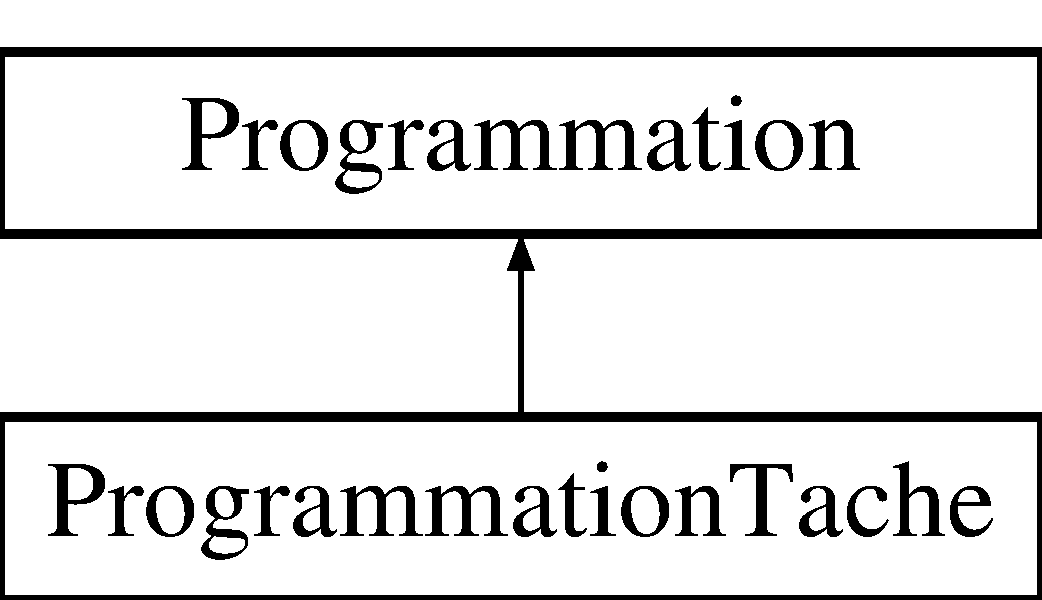
\includegraphics[height=2.000000cm]{class_programmation_tache}
\end{center}
\end{figure}
\subsection*{Public Member Functions}
\begin{DoxyCompactItemize}
\item 
\hyperlink{class_tache_unitaire}{Tache\+Unitaire} $\ast$ \hyperlink{class_programmation_tache_a768420cbc2955fbd0fa4d51651e883f0}{get\+Tache} () const 
\end{DoxyCompactItemize}
\subsection*{Private Member Functions}
\begin{DoxyCompactItemize}
\item 
\hyperlink{class_programmation_tache_a3e3ed2c9849c76f431ad9ae80e1832a9}{Programmation\+Tache} (Q\+String id, Q\+Date dat, int hd, int hf, \hyperlink{class_tache_unitaire}{Tache\+Unitaire} $\ast$ta)
\item 
virtual \hyperlink{class_programmation_tache_a3dae2689c0f94e4f33dd19a7362e498c}{$\sim$\+Programmation\+Tache} ()
\end{DoxyCompactItemize}
\subsection*{Private Attributes}
\begin{DoxyCompactItemize}
\item 
\hyperlink{class_tache_unitaire}{Tache\+Unitaire} $\ast$ \hyperlink{class_programmation_tache_a107df0f6b1dca79ca0b83739d8d177dc}{tache}
\end{DoxyCompactItemize}
\subsection*{Friends}
\begin{DoxyCompactItemize}
\item 
class \hyperlink{class_programmation_tache_ade7bfcbf8cec66b12064c8ff25993d73}{Programmation\+Manager}
\end{DoxyCompactItemize}
\subsection*{Additional Inherited Members}


\subsection{Detailed Description}
Classe représentant une \hyperlink{class_programmation_tache}{Programmation\+Tache}. 

Une \hyperlink{class_programmation_tache}{Programmation\+Tache} est un événement et donc une \hyperlink{class_programmation}{Programmation}. \hyperlink{class_programmation_tache}{Programmation\+Tache} hérite donc de \hyperlink{class_programmation}{Programmation}. Elle est la programmation d\textquotesingle{}une \hyperlink{class_tache}{Tache} donnée. 

\subsection{Constructor \& Destructor Documentation}
\hypertarget{class_programmation_tache_a3e3ed2c9849c76f431ad9ae80e1832a9}{}\index{Programmation\+Tache@{Programmation\+Tache}!Programmation\+Tache@{Programmation\+Tache}}
\index{Programmation\+Tache@{Programmation\+Tache}!Programmation\+Tache@{Programmation\+Tache}}
\subsubsection[{Programmation\+Tache}]{\setlength{\rightskip}{0pt plus 5cm}Programmation\+Tache\+::\+Programmation\+Tache (
\begin{DoxyParamCaption}
\item[{Q\+String}]{id, }
\item[{Q\+Date}]{dat, }
\item[{int}]{hd, }
\item[{int}]{hf, }
\item[{{\bf Tache\+Unitaire} $\ast$}]{ta}
\end{DoxyParamCaption}
)\hspace{0.3cm}{\ttfamily [private]}}\label{class_programmation_tache_a3e3ed2c9849c76f431ad9ae80e1832a9}
Constructeur \hypertarget{class_programmation_tache_a3dae2689c0f94e4f33dd19a7362e498c}{}\index{Programmation\+Tache@{Programmation\+Tache}!````~Programmation\+Tache@{$\sim$\+Programmation\+Tache}}
\index{````~Programmation\+Tache@{$\sim$\+Programmation\+Tache}!Programmation\+Tache@{Programmation\+Tache}}
\subsubsection[{$\sim$\+Programmation\+Tache}]{\setlength{\rightskip}{0pt plus 5cm}Programmation\+Tache\+::$\sim$\+Programmation\+Tache (
\begin{DoxyParamCaption}
{}
\end{DoxyParamCaption}
)\hspace{0.3cm}{\ttfamily [private]}, {\ttfamily [virtual]}}\label{class_programmation_tache_a3dae2689c0f94e4f33dd19a7362e498c}
Destructeur 

\subsection{Member Function Documentation}
\hypertarget{class_programmation_tache_a768420cbc2955fbd0fa4d51651e883f0}{}\index{Programmation\+Tache@{Programmation\+Tache}!get\+Tache@{get\+Tache}}
\index{get\+Tache@{get\+Tache}!Programmation\+Tache@{Programmation\+Tache}}
\subsubsection[{get\+Tache}]{\setlength{\rightskip}{0pt plus 5cm}{\bf Tache\+Unitaire}$\ast$ Programmation\+Tache\+::get\+Tache (
\begin{DoxyParamCaption}
{}
\end{DoxyParamCaption}
) const\hspace{0.3cm}{\ttfamily [inline]}}\label{class_programmation_tache_a768420cbc2955fbd0fa4d51651e883f0}
Renvoie la \hyperlink{class_tache}{Tache} programmée par une \hyperlink{class_programmation_tache}{Programmation\+Tache} 

\subsection{Friends And Related Function Documentation}
\hypertarget{class_programmation_tache_ade7bfcbf8cec66b12064c8ff25993d73}{}\index{Programmation\+Tache@{Programmation\+Tache}!Programmation\+Manager@{Programmation\+Manager}}
\index{Programmation\+Manager@{Programmation\+Manager}!Programmation\+Tache@{Programmation\+Tache}}
\subsubsection[{Programmation\+Manager}]{\setlength{\rightskip}{0pt plus 5cm}friend class {\bf Programmation\+Manager}\hspace{0.3cm}{\ttfamily [friend]}}\label{class_programmation_tache_ade7bfcbf8cec66b12064c8ff25993d73}


\subsection{Member Data Documentation}
\hypertarget{class_programmation_tache_a107df0f6b1dca79ca0b83739d8d177dc}{}\index{Programmation\+Tache@{Programmation\+Tache}!tache@{tache}}
\index{tache@{tache}!Programmation\+Tache@{Programmation\+Tache}}
\subsubsection[{tache}]{\setlength{\rightskip}{0pt plus 5cm}{\bf Tache\+Unitaire}$\ast$ Programmation\+Tache\+::tache\hspace{0.3cm}{\ttfamily [private]}}\label{class_programmation_tache_a107df0f6b1dca79ca0b83739d8d177dc}
\hyperlink{class_tache}{Tache} programmée par une \hyperlink{class_programmation_tache}{Programmation\+Tache} 

The documentation for this class was generated from the following files\+:\begin{DoxyCompactItemize}
\item 
projet/\hyperlink{programmationtache_8h}{programmationtache.\+h}\item 
projet/\hyperlink{programmationtache_8cpp}{programmationtache.\+cpp}\end{DoxyCompactItemize}

\hypertarget{class_projet}{}\section{Référence de la classe Projet}
\label{class_projet}\index{Projet@{Projet}}


{\ttfamily \#include $<$projet.\+h$>$}

\subsection*{Fonctions membres publiques}
\begin{DoxyCompactItemize}
\item 
Q\+String \hyperlink{class_projet_aafdae1361272085ee8683738d70d0612}{get\+Titre} () const 
\item 
Q\+String \hyperlink{class_projet_a4b939075b8f652846f8fc6457343219e}{get\+Description} () const 
\item 
Q\+Vector$<$ \hyperlink{class_tache}{Tache} $\ast$ $>$ \hyperlink{class_projet_abc5c0c5980be9a1639651dc23789f068}{get\+Liste\+Taches} () const 
\item 
Q\+Date \hyperlink{class_projet_a226d910000aaecf7e44399f2226496f5}{get\+Date\+Dispo} () const 
\item 
Q\+Date \hyperlink{class_projet_a6a54a69a00cbaebd362e02f8e7dc3803}{get\+Date\+Echeance} () const 
\item 
\hyperlink{class_tache}{Tache} $\ast$ \hyperlink{class_projet_a4bd470370df8fd883386069a90b958e2}{get\+Tache} (const Q\+String \&id)
\item 
\hyperlink{class_tache_unitaire}{Tache\+Unitaire} $\ast$ \hyperlink{class_projet_a3dfe2bda911378a958b57a6684624804}{add\+Tache\+Unitaire} (const Q\+String \&id, const Q\+String \&tit, const Q\+String \&desc, const int dur, const bool pre)
\item 
\hyperlink{class_tache_unitaire}{Tache\+Unitaire} $\ast$ \hyperlink{class_projet_a8434e7255cace66ff199cb0ba6636535}{add\+Tache\+Unitaire} (const Q\+String \&id, const Q\+String \&tit, const Q\+String \&desc, const Q\+Date \&dd, const Q\+Date \&de, const int dur, const bool pre)
\item 
\hyperlink{class_tache_composite}{Tache\+Composite} $\ast$ \hyperlink{class_projet_aa5f49aee0f30445f1e612311848b78ba}{add\+Tache\+Composite} (const Q\+String \&id, const Q\+String \&tit, const Q\+String \&desc)
\item 
\hyperlink{class_tache_composite}{Tache\+Composite} $\ast$ \hyperlink{class_projet_aee6a754a368eb0ea47b2fa7317ea5055}{add\+Tache\+Composite} (const Q\+String \&id, const Q\+String \&tit, const Q\+String \&desc, const Q\+Date \&dd, const Q\+Date \&de)
\item 
void \hyperlink{class_projet_a649b8123c195bc575871576c9f350d14}{supp\+Tache} (\hyperlink{class_tache_unitaire}{Tache\+Unitaire} $\ast$tache)
\item 
void \hyperlink{class_projet_a1af5c7716e8893066418afc5e8c09f3c}{supp\+Tache} (\hyperlink{class_tache_composite}{Tache\+Composite} $\ast$tache)
\end{DoxyCompactItemize}
\subsection*{Fonctions membres privées}
\begin{DoxyCompactItemize}
\item 
\hyperlink{class_projet_a0149f821f689f5910c7c6d0278d3dd4b}{Projet} (const Q\+String \&t, const Q\+String \&d)
\item 
\hyperlink{class_projet_a26e3e136385eca01dda79df7fba4e03d}{$\sim$\+Projet} ()
\end{DoxyCompactItemize}
\subsection*{Attributs privés}
\begin{DoxyCompactItemize}
\item 
Q\+String \hyperlink{class_projet_a9759849c856c2ac63f94751b876fd289}{titre}
\item 
Q\+String \hyperlink{class_projet_ac2e3a37d5f0201390991b97f258ce0eb}{description}
\item 
Q\+Date \hyperlink{class_projet_a8a89803d629bb571062921008e6a2639}{date\+Dispo}
\item 
Q\+Date \hyperlink{class_projet_a868ee370bb8f071b830dda61f55d99cd}{date\+Echeance}
\item 
Q\+Vector$<$ \hyperlink{class_tache}{Tache} $\ast$ $>$ \hyperlink{class_projet_a268bc6fc9be6d5e266439cc6371cd617}{liste\+Taches}
\end{DoxyCompactItemize}
\subsection*{Amis}
\begin{DoxyCompactItemize}
\item 
class \hyperlink{class_projet_aaaed9857b3481233fa7c581b5c86151d}{Projet\+Manager}
\end{DoxyCompactItemize}


\subsection{Documentation des constructeurs et destructeur}
\hypertarget{class_projet_a0149f821f689f5910c7c6d0278d3dd4b}{}\index{Projet@{Projet}!Projet@{Projet}}
\index{Projet@{Projet}!Projet@{Projet}}
\subsubsection[{Projet}]{\setlength{\rightskip}{0pt plus 5cm}Projet\+::\+Projet (
\begin{DoxyParamCaption}
\item[{const Q\+String \&}]{t, }
\item[{const Q\+String \&}]{d}
\end{DoxyParamCaption}
)\hspace{0.3cm}{\ttfamily [private]}}\label{class_projet_a0149f821f689f5910c7c6d0278d3dd4b}
\hypertarget{class_projet_a26e3e136385eca01dda79df7fba4e03d}{}\index{Projet@{Projet}!````~Projet@{$\sim$\+Projet}}
\index{````~Projet@{$\sim$\+Projet}!Projet@{Projet}}
\subsubsection[{$\sim$\+Projet}]{\setlength{\rightskip}{0pt plus 5cm}Projet\+::$\sim$\+Projet (
\begin{DoxyParamCaption}
{}
\end{DoxyParamCaption}
)\hspace{0.3cm}{\ttfamily [private]}}\label{class_projet_a26e3e136385eca01dda79df7fba4e03d}


\subsection{Documentation des fonctions membres}
\hypertarget{class_projet_aa5f49aee0f30445f1e612311848b78ba}{}\index{Projet@{Projet}!add\+Tache\+Composite@{add\+Tache\+Composite}}
\index{add\+Tache\+Composite@{add\+Tache\+Composite}!Projet@{Projet}}
\subsubsection[{add\+Tache\+Composite}]{\setlength{\rightskip}{0pt plus 5cm}{\bf Tache\+Composite} $\ast$ Projet\+::add\+Tache\+Composite (
\begin{DoxyParamCaption}
\item[{const Q\+String \&}]{id, }
\item[{const Q\+String \&}]{tit, }
\item[{const Q\+String \&}]{desc}
\end{DoxyParamCaption}
)}\label{class_projet_aa5f49aee0f30445f1e612311848b78ba}
\hypertarget{class_projet_aee6a754a368eb0ea47b2fa7317ea5055}{}\index{Projet@{Projet}!add\+Tache\+Composite@{add\+Tache\+Composite}}
\index{add\+Tache\+Composite@{add\+Tache\+Composite}!Projet@{Projet}}
\subsubsection[{add\+Tache\+Composite}]{\setlength{\rightskip}{0pt plus 5cm}{\bf Tache\+Composite} $\ast$ Projet\+::add\+Tache\+Composite (
\begin{DoxyParamCaption}
\item[{const Q\+String \&}]{id, }
\item[{const Q\+String \&}]{tit, }
\item[{const Q\+String \&}]{desc, }
\item[{const Q\+Date \&}]{dd, }
\item[{const Q\+Date \&}]{de}
\end{DoxyParamCaption}
)}\label{class_projet_aee6a754a368eb0ea47b2fa7317ea5055}
\hypertarget{class_projet_a3dfe2bda911378a958b57a6684624804}{}\index{Projet@{Projet}!add\+Tache\+Unitaire@{add\+Tache\+Unitaire}}
\index{add\+Tache\+Unitaire@{add\+Tache\+Unitaire}!Projet@{Projet}}
\subsubsection[{add\+Tache\+Unitaire}]{\setlength{\rightskip}{0pt plus 5cm}{\bf Tache\+Unitaire} $\ast$ Projet\+::add\+Tache\+Unitaire (
\begin{DoxyParamCaption}
\item[{const Q\+String \&}]{id, }
\item[{const Q\+String \&}]{tit, }
\item[{const Q\+String \&}]{desc, }
\item[{const int}]{dur, }
\item[{const bool}]{pre}
\end{DoxyParamCaption}
)}\label{class_projet_a3dfe2bda911378a958b57a6684624804}
\hypertarget{class_projet_a8434e7255cace66ff199cb0ba6636535}{}\index{Projet@{Projet}!add\+Tache\+Unitaire@{add\+Tache\+Unitaire}}
\index{add\+Tache\+Unitaire@{add\+Tache\+Unitaire}!Projet@{Projet}}
\subsubsection[{add\+Tache\+Unitaire}]{\setlength{\rightskip}{0pt plus 5cm}{\bf Tache\+Unitaire} $\ast$ Projet\+::add\+Tache\+Unitaire (
\begin{DoxyParamCaption}
\item[{const Q\+String \&}]{id, }
\item[{const Q\+String \&}]{tit, }
\item[{const Q\+String \&}]{desc, }
\item[{const Q\+Date \&}]{dd, }
\item[{const Q\+Date \&}]{de, }
\item[{const int}]{dur, }
\item[{const bool}]{pre}
\end{DoxyParamCaption}
)}\label{class_projet_a8434e7255cace66ff199cb0ba6636535}
\hypertarget{class_projet_a226d910000aaecf7e44399f2226496f5}{}\index{Projet@{Projet}!get\+Date\+Dispo@{get\+Date\+Dispo}}
\index{get\+Date\+Dispo@{get\+Date\+Dispo}!Projet@{Projet}}
\subsubsection[{get\+Date\+Dispo}]{\setlength{\rightskip}{0pt plus 5cm}Q\+Date Projet\+::get\+Date\+Dispo (
\begin{DoxyParamCaption}
{}
\end{DoxyParamCaption}
) const\hspace{0.3cm}{\ttfamily [inline]}}\label{class_projet_a226d910000aaecf7e44399f2226496f5}
\hypertarget{class_projet_a6a54a69a00cbaebd362e02f8e7dc3803}{}\index{Projet@{Projet}!get\+Date\+Echeance@{get\+Date\+Echeance}}
\index{get\+Date\+Echeance@{get\+Date\+Echeance}!Projet@{Projet}}
\subsubsection[{get\+Date\+Echeance}]{\setlength{\rightskip}{0pt plus 5cm}Q\+Date Projet\+::get\+Date\+Echeance (
\begin{DoxyParamCaption}
{}
\end{DoxyParamCaption}
) const\hspace{0.3cm}{\ttfamily [inline]}}\label{class_projet_a6a54a69a00cbaebd362e02f8e7dc3803}
\hypertarget{class_projet_a4b939075b8f652846f8fc6457343219e}{}\index{Projet@{Projet}!get\+Description@{get\+Description}}
\index{get\+Description@{get\+Description}!Projet@{Projet}}
\subsubsection[{get\+Description}]{\setlength{\rightskip}{0pt plus 5cm}Q\+String Projet\+::get\+Description (
\begin{DoxyParamCaption}
{}
\end{DoxyParamCaption}
) const\hspace{0.3cm}{\ttfamily [inline]}}\label{class_projet_a4b939075b8f652846f8fc6457343219e}
\hypertarget{class_projet_abc5c0c5980be9a1639651dc23789f068}{}\index{Projet@{Projet}!get\+Liste\+Taches@{get\+Liste\+Taches}}
\index{get\+Liste\+Taches@{get\+Liste\+Taches}!Projet@{Projet}}
\subsubsection[{get\+Liste\+Taches}]{\setlength{\rightskip}{0pt plus 5cm}Q\+Vector$<${\bf Tache}$\ast$$>$ Projet\+::get\+Liste\+Taches (
\begin{DoxyParamCaption}
{}
\end{DoxyParamCaption}
) const\hspace{0.3cm}{\ttfamily [inline]}}\label{class_projet_abc5c0c5980be9a1639651dc23789f068}
\hypertarget{class_projet_a4bd470370df8fd883386069a90b958e2}{}\index{Projet@{Projet}!get\+Tache@{get\+Tache}}
\index{get\+Tache@{get\+Tache}!Projet@{Projet}}
\subsubsection[{get\+Tache}]{\setlength{\rightskip}{0pt plus 5cm}{\bf Tache} $\ast$ Projet\+::get\+Tache (
\begin{DoxyParamCaption}
\item[{const Q\+String \&}]{id}
\end{DoxyParamCaption}
)}\label{class_projet_a4bd470370df8fd883386069a90b958e2}
\hypertarget{class_projet_aafdae1361272085ee8683738d70d0612}{}\index{Projet@{Projet}!get\+Titre@{get\+Titre}}
\index{get\+Titre@{get\+Titre}!Projet@{Projet}}
\subsubsection[{get\+Titre}]{\setlength{\rightskip}{0pt plus 5cm}Q\+String Projet\+::get\+Titre (
\begin{DoxyParamCaption}
{}
\end{DoxyParamCaption}
) const\hspace{0.3cm}{\ttfamily [inline]}}\label{class_projet_aafdae1361272085ee8683738d70d0612}
\hypertarget{class_projet_a649b8123c195bc575871576c9f350d14}{}\index{Projet@{Projet}!supp\+Tache@{supp\+Tache}}
\index{supp\+Tache@{supp\+Tache}!Projet@{Projet}}
\subsubsection[{supp\+Tache}]{\setlength{\rightskip}{0pt plus 5cm}void Projet\+::supp\+Tache (
\begin{DoxyParamCaption}
\item[{{\bf Tache\+Unitaire} $\ast$}]{tache}
\end{DoxyParamCaption}
)}\label{class_projet_a649b8123c195bc575871576c9f350d14}
\hypertarget{class_projet_a1af5c7716e8893066418afc5e8c09f3c}{}\index{Projet@{Projet}!supp\+Tache@{supp\+Tache}}
\index{supp\+Tache@{supp\+Tache}!Projet@{Projet}}
\subsubsection[{supp\+Tache}]{\setlength{\rightskip}{0pt plus 5cm}void Projet\+::supp\+Tache (
\begin{DoxyParamCaption}
\item[{{\bf Tache\+Composite} $\ast$}]{tache}
\end{DoxyParamCaption}
)}\label{class_projet_a1af5c7716e8893066418afc5e8c09f3c}


\subsection{Documentation des fonctions amies et associées}
\hypertarget{class_projet_aaaed9857b3481233fa7c581b5c86151d}{}\index{Projet@{Projet}!Projet\+Manager@{Projet\+Manager}}
\index{Projet\+Manager@{Projet\+Manager}!Projet@{Projet}}
\subsubsection[{Projet\+Manager}]{\setlength{\rightskip}{0pt plus 5cm}friend class {\bf Projet\+Manager}\hspace{0.3cm}{\ttfamily [friend]}}\label{class_projet_aaaed9857b3481233fa7c581b5c86151d}


\subsection{Documentation des données membres}
\hypertarget{class_projet_a8a89803d629bb571062921008e6a2639}{}\index{Projet@{Projet}!date\+Dispo@{date\+Dispo}}
\index{date\+Dispo@{date\+Dispo}!Projet@{Projet}}
\subsubsection[{date\+Dispo}]{\setlength{\rightskip}{0pt plus 5cm}Q\+Date Projet\+::date\+Dispo\hspace{0.3cm}{\ttfamily [private]}}\label{class_projet_a8a89803d629bb571062921008e6a2639}
\hypertarget{class_projet_a868ee370bb8f071b830dda61f55d99cd}{}\index{Projet@{Projet}!date\+Echeance@{date\+Echeance}}
\index{date\+Echeance@{date\+Echeance}!Projet@{Projet}}
\subsubsection[{date\+Echeance}]{\setlength{\rightskip}{0pt plus 5cm}Q\+Date Projet\+::date\+Echeance\hspace{0.3cm}{\ttfamily [private]}}\label{class_projet_a868ee370bb8f071b830dda61f55d99cd}
\hypertarget{class_projet_ac2e3a37d5f0201390991b97f258ce0eb}{}\index{Projet@{Projet}!description@{description}}
\index{description@{description}!Projet@{Projet}}
\subsubsection[{description}]{\setlength{\rightskip}{0pt plus 5cm}Q\+String Projet\+::description\hspace{0.3cm}{\ttfamily [private]}}\label{class_projet_ac2e3a37d5f0201390991b97f258ce0eb}
\hypertarget{class_projet_a268bc6fc9be6d5e266439cc6371cd617}{}\index{Projet@{Projet}!liste\+Taches@{liste\+Taches}}
\index{liste\+Taches@{liste\+Taches}!Projet@{Projet}}
\subsubsection[{liste\+Taches}]{\setlength{\rightskip}{0pt plus 5cm}Q\+Vector$<${\bf Tache}$\ast$$>$ Projet\+::liste\+Taches\hspace{0.3cm}{\ttfamily [private]}}\label{class_projet_a268bc6fc9be6d5e266439cc6371cd617}
\hypertarget{class_projet_a9759849c856c2ac63f94751b876fd289}{}\index{Projet@{Projet}!titre@{titre}}
\index{titre@{titre}!Projet@{Projet}}
\subsubsection[{titre}]{\setlength{\rightskip}{0pt plus 5cm}Q\+String Projet\+::titre\hspace{0.3cm}{\ttfamily [private]}}\label{class_projet_a9759849c856c2ac63f94751b876fd289}


La documentation de cette classe a été générée à partir des fichiers suivants \+:\begin{DoxyCompactItemize}
\item 
\hyperlink{projet_8h}{projet.\+h}\item 
\hyperlink{projet_8cpp}{projet.\+cpp}\end{DoxyCompactItemize}

\hypertarget{class_projet_manager}{}\section{Projet\+Manager Class Reference}
\label{class_projet_manager}\index{Projet\+Manager@{Projet\+Manager}}


Classe représentant le manager de projet.  




{\ttfamily \#include $<$projetmanager.\+h$>$}

\subsection*{Public Member Functions}
\begin{DoxyCompactItemize}
\item 
Q\+Vector$<$ \hyperlink{class_projet}{Projet} $\ast$ $>$ \hyperlink{class_projet_manager_a2b7281842b818a8e2cd85a81ef270930}{get\+Liste\+Projet} () const 
\item 
\hyperlink{class_projet}{Projet} $\ast$ \hyperlink{class_projet_manager_a1c547839afb77faaa3eb2f37e0c869a7}{add\+Projet} (const Q\+String \&t, const Q\+String \&d)
\item 
void \hyperlink{class_projet_manager_a7c76e23d621d3e904e3e2a1bdc4c176c}{supp\+Projet} (\hyperlink{class_projet}{Projet} $\ast$projet)
\end{DoxyCompactItemize}
\subsection*{Static Public Member Functions}
\begin{DoxyCompactItemize}
\item 
static \hyperlink{class_projet_manager}{Projet\+Manager} \& \hyperlink{class_projet_manager_ad61417127cad478ea812d560b18b975d}{Instance} ()
\end{DoxyCompactItemize}
\subsection*{Private Member Functions}
\begin{DoxyCompactItemize}
\item 
\hyperlink{class_projet_manager_a98d8ba59bd9bc6eec2ec5285102ac9a1}{Projet\+Manager} ()
\item 
\hyperlink{class_projet_manager_af5a44cde2f8d92f05bb7e52a18aa883a}{$\sim$\+Projet\+Manager} ()
\item 
\hyperlink{class_projet_manager}{Projet\+Manager} \& \hyperlink{class_projet_manager_a25b560fb4e617952ad093bbe74315aaa}{operator=} (const \hyperlink{class_projet_manager}{Projet\+Manager} \&)
\item 
\hyperlink{class_projet_manager_abfdc065f2c1819e13c8adc1562536f35}{Projet\+Manager} (const \hyperlink{class_projet_manager}{Projet\+Manager} \&)
\end{DoxyCompactItemize}
\subsection*{Private Attributes}
\begin{DoxyCompactItemize}
\item 
Q\+Vector$<$ \hyperlink{class_projet}{Projet} $\ast$ $>$ \hyperlink{class_projet_manager_a46c2e5dab1e538225fa022030e3a31d1}{liste\+Projets}
\end{DoxyCompactItemize}
\subsection*{Static Private Attributes}
\begin{DoxyCompactItemize}
\item 
static \hyperlink{class_projet_manager}{Projet\+Manager} \hyperlink{class_projet_manager_a88d70fa1123219b8dbb749818a441afa}{instance} =\hyperlink{class_projet_manager}{Projet\+Manager}()
\end{DoxyCompactItemize}


\subsection{Detailed Description}
Classe représentant le manager de projet. 

Le manager de projet est unique et ne doit être instancié qu\textquotesingle{}une seule fois. Il utilise donc le design pattern singleton. Il y a une composition entre \hyperlink{class_projet_manager}{Projet\+Manager} et \hyperlink{class_projet}{Projet}. En effet, \hyperlink{class_projet_manager}{Projet\+Manager} détermine la durée de vie d\textquotesingle{}un \hyperlink{class_projet}{Projet}. 

\subsection{Constructor \& Destructor Documentation}
\hypertarget{class_projet_manager_a98d8ba59bd9bc6eec2ec5285102ac9a1}{}\index{Projet\+Manager@{Projet\+Manager}!Projet\+Manager@{Projet\+Manager}}
\index{Projet\+Manager@{Projet\+Manager}!Projet\+Manager@{Projet\+Manager}}
\subsubsection[{Projet\+Manager}]{\setlength{\rightskip}{0pt plus 5cm}Projet\+Manager\+::\+Projet\+Manager (
\begin{DoxyParamCaption}
{}
\end{DoxyParamCaption}
)\hspace{0.3cm}{\ttfamily [private]}}\label{class_projet_manager_a98d8ba59bd9bc6eec2ec5285102ac9a1}
Constructeur \hypertarget{class_projet_manager_af5a44cde2f8d92f05bb7e52a18aa883a}{}\index{Projet\+Manager@{Projet\+Manager}!````~Projet\+Manager@{$\sim$\+Projet\+Manager}}
\index{````~Projet\+Manager@{$\sim$\+Projet\+Manager}!Projet\+Manager@{Projet\+Manager}}
\subsubsection[{$\sim$\+Projet\+Manager}]{\setlength{\rightskip}{0pt plus 5cm}Projet\+Manager\+::$\sim$\+Projet\+Manager (
\begin{DoxyParamCaption}
{}
\end{DoxyParamCaption}
)\hspace{0.3cm}{\ttfamily [private]}}\label{class_projet_manager_af5a44cde2f8d92f05bb7e52a18aa883a}
Destructeur \hypertarget{class_projet_manager_abfdc065f2c1819e13c8adc1562536f35}{}\index{Projet\+Manager@{Projet\+Manager}!Projet\+Manager@{Projet\+Manager}}
\index{Projet\+Manager@{Projet\+Manager}!Projet\+Manager@{Projet\+Manager}}
\subsubsection[{Projet\+Manager}]{\setlength{\rightskip}{0pt plus 5cm}Projet\+Manager\+::\+Projet\+Manager (
\begin{DoxyParamCaption}
\item[{const {\bf Projet\+Manager} \&}]{}
\end{DoxyParamCaption}
)\hspace{0.3cm}{\ttfamily [inline]}, {\ttfamily [private]}}\label{class_projet_manager_abfdc065f2c1819e13c8adc1562536f35}
Constructeur par recopie 

\subsection{Member Function Documentation}
\hypertarget{class_projet_manager_a1c547839afb77faaa3eb2f37e0c869a7}{}\index{Projet\+Manager@{Projet\+Manager}!add\+Projet@{add\+Projet}}
\index{add\+Projet@{add\+Projet}!Projet\+Manager@{Projet\+Manager}}
\subsubsection[{add\+Projet}]{\setlength{\rightskip}{0pt plus 5cm}{\bf Projet} $\ast$ Projet\+Manager\+::add\+Projet (
\begin{DoxyParamCaption}
\item[{const Q\+String \&}]{t, }
\item[{const Q\+String \&}]{d}
\end{DoxyParamCaption}
)}\label{class_projet_manager_a1c547839afb77faaa3eb2f37e0c869a7}
Créer et ajoute un \hyperlink{class_projet}{Projet} \hypertarget{class_projet_manager_a2b7281842b818a8e2cd85a81ef270930}{}\index{Projet\+Manager@{Projet\+Manager}!get\+Liste\+Projet@{get\+Liste\+Projet}}
\index{get\+Liste\+Projet@{get\+Liste\+Projet}!Projet\+Manager@{Projet\+Manager}}
\subsubsection[{get\+Liste\+Projet}]{\setlength{\rightskip}{0pt plus 5cm}Q\+Vector$<${\bf Projet}$\ast$$>$ Projet\+Manager\+::get\+Liste\+Projet (
\begin{DoxyParamCaption}
{}
\end{DoxyParamCaption}
) const\hspace{0.3cm}{\ttfamily [inline]}}\label{class_projet_manager_a2b7281842b818a8e2cd85a81ef270930}
Renvoie un vecteur contenant tous les projets \hypertarget{class_projet_manager_ad61417127cad478ea812d560b18b975d}{}\index{Projet\+Manager@{Projet\+Manager}!Instance@{Instance}}
\index{Instance@{Instance}!Projet\+Manager@{Projet\+Manager}}
\subsubsection[{Instance}]{\setlength{\rightskip}{0pt plus 5cm}{\bf Projet\+Manager} \& Projet\+Manager\+::\+Instance (
\begin{DoxyParamCaption}
{}
\end{DoxyParamCaption}
)\hspace{0.3cm}{\ttfamily [static]}}\label{class_projet_manager_ad61417127cad478ea812d560b18b975d}
Instancie \hyperlink{class_projet_manager}{Projet\+Manager} \hypertarget{class_projet_manager_a25b560fb4e617952ad093bbe74315aaa}{}\index{Projet\+Manager@{Projet\+Manager}!operator=@{operator=}}
\index{operator=@{operator=}!Projet\+Manager@{Projet\+Manager}}
\subsubsection[{operator=}]{\setlength{\rightskip}{0pt plus 5cm}{\bf Projet\+Manager}\& Projet\+Manager\+::operator= (
\begin{DoxyParamCaption}
\item[{const {\bf Projet\+Manager} \&}]{}
\end{DoxyParamCaption}
)\hspace{0.3cm}{\ttfamily [inline]}, {\ttfamily [private]}}\label{class_projet_manager_a25b560fb4e617952ad093bbe74315aaa}
Opérateur de recopie \hypertarget{class_projet_manager_a7c76e23d621d3e904e3e2a1bdc4c176c}{}\index{Projet\+Manager@{Projet\+Manager}!supp\+Projet@{supp\+Projet}}
\index{supp\+Projet@{supp\+Projet}!Projet\+Manager@{Projet\+Manager}}
\subsubsection[{supp\+Projet}]{\setlength{\rightskip}{0pt plus 5cm}void Projet\+Manager\+::supp\+Projet (
\begin{DoxyParamCaption}
\item[{{\bf Projet} $\ast$}]{projet}
\end{DoxyParamCaption}
)}\label{class_projet_manager_a7c76e23d621d3e904e3e2a1bdc4c176c}
Détruit un \hyperlink{class_projet}{Projet} 

\subsection{Member Data Documentation}
\hypertarget{class_projet_manager_a88d70fa1123219b8dbb749818a441afa}{}\index{Projet\+Manager@{Projet\+Manager}!instance@{instance}}
\index{instance@{instance}!Projet\+Manager@{Projet\+Manager}}
\subsubsection[{instance}]{\setlength{\rightskip}{0pt plus 5cm}{\bf Projet\+Manager} Projet\+Manager\+::instance ={\bf Projet\+Manager}()\hspace{0.3cm}{\ttfamily [static]}, {\ttfamily [private]}}\label{class_projet_manager_a88d70fa1123219b8dbb749818a441afa}
Instance unique de \hyperlink{class_projet_manager}{Projet\+Manager} \hypertarget{class_projet_manager_a46c2e5dab1e538225fa022030e3a31d1}{}\index{Projet\+Manager@{Projet\+Manager}!liste\+Projets@{liste\+Projets}}
\index{liste\+Projets@{liste\+Projets}!Projet\+Manager@{Projet\+Manager}}
\subsubsection[{liste\+Projets}]{\setlength{\rightskip}{0pt plus 5cm}Q\+Vector$<${\bf Projet}$\ast$$>$ Projet\+Manager\+::liste\+Projets\hspace{0.3cm}{\ttfamily [private]}}\label{class_projet_manager_a46c2e5dab1e538225fa022030e3a31d1}
Vecteur de tous les \hyperlink{class_projet}{Projet} 

The documentation for this class was generated from the following files\+:\begin{DoxyCompactItemize}
\item 
projet/\hyperlink{projetmanager_8h}{projetmanager.\+h}\item 
projet/\hyperlink{projetmanager_8cpp}{projetmanager.\+cpp}\end{DoxyCompactItemize}

\hypertarget{class_tache}{}\section{Tache Class Reference}
\label{class_tache}\index{Tache@{Tache}}


Classe représentant une tâche.  




{\ttfamily \#include $<$tache.\+h$>$}

Inheritance diagram for Tache\+:\begin{figure}[H]
\begin{center}
\leavevmode
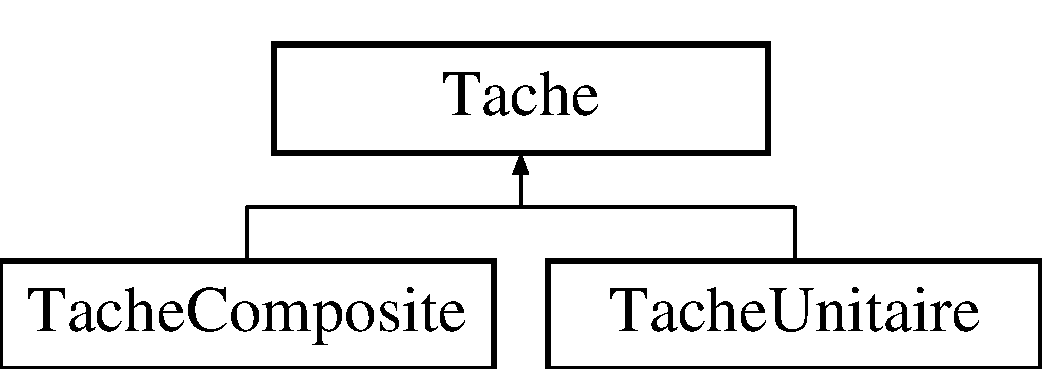
\includegraphics[height=2.000000cm]{class_tache}
\end{center}
\end{figure}
\subsection*{Public Member Functions}
\begin{DoxyCompactItemize}
\item 
\hyperlink{class_projet}{Projet} $\ast$ \hyperlink{class_tache_aa6d1abc3712b5a8b571bb3c131129ac7}{get\+Projet} () const 
\item 
Q\+String \hyperlink{class_tache_aff63994ef1fe1b96cf14540f954e45c0}{get\+Identifiant} () const 
\item 
Q\+String \hyperlink{class_tache_ab9e56c6eaaa23d2c66148ff5a89724e6}{get\+Titre} () const 
\item 
Q\+String \hyperlink{class_tache_a02954f46ea1310fb0d5ceceeb94298cc}{get\+Description} () const 
\item 
Q\+Date \hyperlink{class_tache_a5f7e485d64f7e72042e1f0ad5f378df4}{get\+Date\+Dispo} () const 
\item 
Q\+Date \hyperlink{class_tache_ad44bf074be085367c3a58b81be680d70}{get\+Date\+Echeance} () const 
\item 
\hyperlink{class_tache_composite}{Tache\+Composite} $\ast$ \hyperlink{class_tache_a5d8c5f16db0287ed0539c9206f244e02}{get\+Tache\+Mere\+Composite} () const 
\item 
Q\+Vector$<$ \hyperlink{class_tache}{Tache} $\ast$ $>$ \hyperlink{class_tache_afa1e10f04b303908477feee22241820f}{get\+Liste\+Taches\+Meres\+Precedence} () const 
\item 
void \hyperlink{class_tache_ad5ed4f92ccbc0895813908c750d918a2}{set\+Tache\+Mere\+Composite} (\hyperlink{class_tache_composite}{Tache\+Composite} $\ast$mere)
\item 
void \hyperlink{class_tache_a10659477f457bc4ceafbee41b155eb66}{add\+Precedence} (\hyperlink{class_tache}{Tache} $\ast$precedence)
\end{DoxyCompactItemize}
\subsection*{Protected Member Functions}
\begin{DoxyCompactItemize}
\item 
\hyperlink{class_tache_af712b59bd6e56adc46904a6445431ae7}{Tache} (const Q\+String \&id, const Q\+String \&t, const Q\+String \&d, \hyperlink{class_projet}{Projet} $\ast$p)
\item 
\hyperlink{class_tache_a5b02c50c65270708b1a18c1a810ca00a}{Tache} (const Q\+String \&id, const Q\+String \&t, const Q\+String \&d, const Q\+Date \&dd, const Q\+Date \&de, \hyperlink{class_projet}{Projet} $\ast$p)
\item 
virtual \hyperlink{class_tache_a7ff832b739f8365acbe60275c7868c63}{$\sim$\+Tache} ()
\item 
bool \hyperlink{class_tache_a579d9a3b88293522b7326e5d11815091}{check\+Precedence} (\hyperlink{class_tache}{Tache} $\ast$precedence)
\item 
void \hyperlink{class_tache_a00babe6049701a1148eaca5336454731}{supp\+Precedence} (\hyperlink{class_tache}{Tache} $\ast$precedence)
\end{DoxyCompactItemize}
\subsection*{Protected Attributes}
\begin{DoxyCompactItemize}
\item 
Q\+String \hyperlink{class_tache_a9af1773c9b835900bba8814cccee450e}{identifiant}
\item 
Q\+String \hyperlink{class_tache_a1d3d20046c0c4cc8482f71bb555b79cf}{titre}
\item 
Q\+String \hyperlink{class_tache_ab3d06410b2c62ebfbe20f570c41dc4d4}{description}
\item 
Q\+Date \hyperlink{class_tache_ac8758b826b1be639dad8bcb556659a36}{date\+Dispo}
\item 
Q\+Date \hyperlink{class_tache_a7671c127da40ae35075f069a64396f45}{date\+Echeance}
\item 
Q\+Vector$<$ \hyperlink{class_tache}{Tache} $\ast$ $>$ \hyperlink{class_tache_a0f73920789e27b7c2aeb47d171d5e543}{liste\+Taches\+Meres\+Precedence}
\item 
\hyperlink{class_tache_composite}{Tache\+Composite} $\ast$ \hyperlink{class_tache_a62e6fe2722630c7bdf9a4a6a42364a19}{tache\+Mere\+Composite}
\item 
\hyperlink{class_projet}{Projet} $\ast$ \hyperlink{class_tache_a0c6d513a2a376b18cb73ab726fe4dec1}{projet}
\end{DoxyCompactItemize}
\subsection*{Friends}
\begin{DoxyCompactItemize}
\item 
class \hyperlink{class_tache_ab87b41c3faa36955cc370972f5cce344}{Projet}
\end{DoxyCompactItemize}


\subsection{Detailed Description}
Classe représentant une tâche. 

Une tâche est forcément associée à un \hyperlink{class_projet}{Projet}. 

\subsection{Constructor \& Destructor Documentation}
\hypertarget{class_tache_af712b59bd6e56adc46904a6445431ae7}{}\index{Tache@{Tache}!Tache@{Tache}}
\index{Tache@{Tache}!Tache@{Tache}}
\subsubsection[{Tache}]{\setlength{\rightskip}{0pt plus 5cm}Tache\+::\+Tache (
\begin{DoxyParamCaption}
\item[{const Q\+String \&}]{id, }
\item[{const Q\+String \&}]{t, }
\item[{const Q\+String \&}]{d, }
\item[{{\bf Projet} $\ast$}]{p}
\end{DoxyParamCaption}
)\hspace{0.3cm}{\ttfamily [protected]}}\label{class_tache_af712b59bd6e56adc46904a6445431ae7}
\hypertarget{class_tache_a5b02c50c65270708b1a18c1a810ca00a}{}\index{Tache@{Tache}!Tache@{Tache}}
\index{Tache@{Tache}!Tache@{Tache}}
\subsubsection[{Tache}]{\setlength{\rightskip}{0pt plus 5cm}Tache\+::\+Tache (
\begin{DoxyParamCaption}
\item[{const Q\+String \&}]{id, }
\item[{const Q\+String \&}]{t, }
\item[{const Q\+String \&}]{d, }
\item[{const Q\+Date \&}]{dd, }
\item[{const Q\+Date \&}]{de, }
\item[{{\bf Projet} $\ast$}]{p}
\end{DoxyParamCaption}
)\hspace{0.3cm}{\ttfamily [protected]}}\label{class_tache_a5b02c50c65270708b1a18c1a810ca00a}
\hypertarget{class_tache_a7ff832b739f8365acbe60275c7868c63}{}\index{Tache@{Tache}!````~Tache@{$\sim$\+Tache}}
\index{````~Tache@{$\sim$\+Tache}!Tache@{Tache}}
\subsubsection[{$\sim$\+Tache}]{\setlength{\rightskip}{0pt plus 5cm}Tache\+::$\sim$\+Tache (
\begin{DoxyParamCaption}
{}
\end{DoxyParamCaption}
)\hspace{0.3cm}{\ttfamily [protected]}, {\ttfamily [virtual]}}\label{class_tache_a7ff832b739f8365acbe60275c7868c63}


\subsection{Member Function Documentation}
\hypertarget{class_tache_a10659477f457bc4ceafbee41b155eb66}{}\index{Tache@{Tache}!add\+Precedence@{add\+Precedence}}
\index{add\+Precedence@{add\+Precedence}!Tache@{Tache}}
\subsubsection[{add\+Precedence}]{\setlength{\rightskip}{0pt plus 5cm}void Tache\+::add\+Precedence (
\begin{DoxyParamCaption}
\item[{{\bf Tache} $\ast$}]{precedence}
\end{DoxyParamCaption}
)}\label{class_tache_a10659477f457bc4ceafbee41b155eb66}
Ajoute une tâche comme précédence d\textquotesingle{}une autre tâche. \hypertarget{class_tache_a579d9a3b88293522b7326e5d11815091}{}\index{Tache@{Tache}!check\+Precedence@{check\+Precedence}}
\index{check\+Precedence@{check\+Precedence}!Tache@{Tache}}
\subsubsection[{check\+Precedence}]{\setlength{\rightskip}{0pt plus 5cm}bool Tache\+::check\+Precedence (
\begin{DoxyParamCaption}
\item[{{\bf Tache} $\ast$}]{precedence}
\end{DoxyParamCaption}
)\hspace{0.3cm}{\ttfamily [protected]}}\label{class_tache_a579d9a3b88293522b7326e5d11815091}
\hypertarget{class_tache_a5f7e485d64f7e72042e1f0ad5f378df4}{}\index{Tache@{Tache}!get\+Date\+Dispo@{get\+Date\+Dispo}}
\index{get\+Date\+Dispo@{get\+Date\+Dispo}!Tache@{Tache}}
\subsubsection[{get\+Date\+Dispo}]{\setlength{\rightskip}{0pt plus 5cm}Q\+Date Tache\+::get\+Date\+Dispo (
\begin{DoxyParamCaption}
{}
\end{DoxyParamCaption}
) const\hspace{0.3cm}{\ttfamily [inline]}}\label{class_tache_a5f7e485d64f7e72042e1f0ad5f378df4}
Retourne ldate de disponibilité d\textquotesingle{}une tâche. \hypertarget{class_tache_ad44bf074be085367c3a58b81be680d70}{}\index{Tache@{Tache}!get\+Date\+Echeance@{get\+Date\+Echeance}}
\index{get\+Date\+Echeance@{get\+Date\+Echeance}!Tache@{Tache}}
\subsubsection[{get\+Date\+Echeance}]{\setlength{\rightskip}{0pt plus 5cm}Q\+Date Tache\+::get\+Date\+Echeance (
\begin{DoxyParamCaption}
{}
\end{DoxyParamCaption}
) const\hspace{0.3cm}{\ttfamily [inline]}}\label{class_tache_ad44bf074be085367c3a58b81be680d70}
Retourne la date d\textquotesingle{}échéance d\textquotesingle{}une tâche. \hypertarget{class_tache_a02954f46ea1310fb0d5ceceeb94298cc}{}\index{Tache@{Tache}!get\+Description@{get\+Description}}
\index{get\+Description@{get\+Description}!Tache@{Tache}}
\subsubsection[{get\+Description}]{\setlength{\rightskip}{0pt plus 5cm}Q\+String Tache\+::get\+Description (
\begin{DoxyParamCaption}
{}
\end{DoxyParamCaption}
) const\hspace{0.3cm}{\ttfamily [inline]}}\label{class_tache_a02954f46ea1310fb0d5ceceeb94298cc}
Retourne la description d\textquotesingle{}une tâche. \hypertarget{class_tache_aff63994ef1fe1b96cf14540f954e45c0}{}\index{Tache@{Tache}!get\+Identifiant@{get\+Identifiant}}
\index{get\+Identifiant@{get\+Identifiant}!Tache@{Tache}}
\subsubsection[{get\+Identifiant}]{\setlength{\rightskip}{0pt plus 5cm}Q\+String Tache\+::get\+Identifiant (
\begin{DoxyParamCaption}
{}
\end{DoxyParamCaption}
) const\hspace{0.3cm}{\ttfamily [inline]}}\label{class_tache_aff63994ef1fe1b96cf14540f954e45c0}
Retourne l\textquotesingle{}identifiant d\textquotesingle{}une tâche. \hypertarget{class_tache_afa1e10f04b303908477feee22241820f}{}\index{Tache@{Tache}!get\+Liste\+Taches\+Meres\+Precedence@{get\+Liste\+Taches\+Meres\+Precedence}}
\index{get\+Liste\+Taches\+Meres\+Precedence@{get\+Liste\+Taches\+Meres\+Precedence}!Tache@{Tache}}
\subsubsection[{get\+Liste\+Taches\+Meres\+Precedence}]{\setlength{\rightskip}{0pt plus 5cm}Q\+Vector$<${\bf Tache}$\ast$$>$ Tache\+::get\+Liste\+Taches\+Meres\+Precedence (
\begin{DoxyParamCaption}
{}
\end{DoxyParamCaption}
) const\hspace{0.3cm}{\ttfamily [inline]}}\label{class_tache_afa1e10f04b303908477feee22241820f}
Retourne une liste de tâche précédant une autre tâche. \hypertarget{class_tache_aa6d1abc3712b5a8b571bb3c131129ac7}{}\index{Tache@{Tache}!get\+Projet@{get\+Projet}}
\index{get\+Projet@{get\+Projet}!Tache@{Tache}}
\subsubsection[{get\+Projet}]{\setlength{\rightskip}{0pt plus 5cm}{\bf Projet}$\ast$ Tache\+::get\+Projet (
\begin{DoxyParamCaption}
{}
\end{DoxyParamCaption}
) const\hspace{0.3cm}{\ttfamily [inline]}}\label{class_tache_aa6d1abc3712b5a8b571bb3c131129ac7}
Retourne le projet d\textquotesingle{}une tâche. \hypertarget{class_tache_a5d8c5f16db0287ed0539c9206f244e02}{}\index{Tache@{Tache}!get\+Tache\+Mere\+Composite@{get\+Tache\+Mere\+Composite}}
\index{get\+Tache\+Mere\+Composite@{get\+Tache\+Mere\+Composite}!Tache@{Tache}}
\subsubsection[{get\+Tache\+Mere\+Composite}]{\setlength{\rightskip}{0pt plus 5cm}{\bf Tache\+Composite}$\ast$ Tache\+::get\+Tache\+Mere\+Composite (
\begin{DoxyParamCaption}
{}
\end{DoxyParamCaption}
) const\hspace{0.3cm}{\ttfamily [inline]}}\label{class_tache_a5d8c5f16db0287ed0539c9206f244e02}
Retourne la tâche dont une tâche est composition. \hypertarget{class_tache_ab9e56c6eaaa23d2c66148ff5a89724e6}{}\index{Tache@{Tache}!get\+Titre@{get\+Titre}}
\index{get\+Titre@{get\+Titre}!Tache@{Tache}}
\subsubsection[{get\+Titre}]{\setlength{\rightskip}{0pt plus 5cm}Q\+String Tache\+::get\+Titre (
\begin{DoxyParamCaption}
{}
\end{DoxyParamCaption}
) const\hspace{0.3cm}{\ttfamily [inline]}}\label{class_tache_ab9e56c6eaaa23d2c66148ff5a89724e6}
Retourne le titre d\textquotesingle{}une tâche. \hypertarget{class_tache_ad5ed4f92ccbc0895813908c750d918a2}{}\index{Tache@{Tache}!set\+Tache\+Mere\+Composite@{set\+Tache\+Mere\+Composite}}
\index{set\+Tache\+Mere\+Composite@{set\+Tache\+Mere\+Composite}!Tache@{Tache}}
\subsubsection[{set\+Tache\+Mere\+Composite}]{\setlength{\rightskip}{0pt plus 5cm}void Tache\+::set\+Tache\+Mere\+Composite (
\begin{DoxyParamCaption}
\item[{{\bf Tache\+Composite} $\ast$}]{mere}
\end{DoxyParamCaption}
)}\label{class_tache_ad5ed4f92ccbc0895813908c750d918a2}
Affecte une tâche en tant que tâche dont une autre tâche est composition. \hypertarget{class_tache_a00babe6049701a1148eaca5336454731}{}\index{Tache@{Tache}!supp\+Precedence@{supp\+Precedence}}
\index{supp\+Precedence@{supp\+Precedence}!Tache@{Tache}}
\subsubsection[{supp\+Precedence}]{\setlength{\rightskip}{0pt plus 5cm}void Tache\+::supp\+Precedence (
\begin{DoxyParamCaption}
\item[{{\bf Tache} $\ast$}]{precedence}
\end{DoxyParamCaption}
)\hspace{0.3cm}{\ttfamily [protected]}}\label{class_tache_a00babe6049701a1148eaca5336454731}


\subsection{Friends And Related Function Documentation}
\hypertarget{class_tache_ab87b41c3faa36955cc370972f5cce344}{}\index{Tache@{Tache}!Projet@{Projet}}
\index{Projet@{Projet}!Tache@{Tache}}
\subsubsection[{Projet}]{\setlength{\rightskip}{0pt plus 5cm}friend class {\bf Projet}\hspace{0.3cm}{\ttfamily [friend]}}\label{class_tache_ab87b41c3faa36955cc370972f5cce344}


\subsection{Member Data Documentation}
\hypertarget{class_tache_ac8758b826b1be639dad8bcb556659a36}{}\index{Tache@{Tache}!date\+Dispo@{date\+Dispo}}
\index{date\+Dispo@{date\+Dispo}!Tache@{Tache}}
\subsubsection[{date\+Dispo}]{\setlength{\rightskip}{0pt plus 5cm}Q\+Date Tache\+::date\+Dispo\hspace{0.3cm}{\ttfamily [protected]}}\label{class_tache_ac8758b826b1be639dad8bcb556659a36}
Date de disponibilité d\textquotesingle{}une tâche. Une tâche ne peut être commencé que lorsque sa date de disponibilité est passée. \hypertarget{class_tache_a7671c127da40ae35075f069a64396f45}{}\index{Tache@{Tache}!date\+Echeance@{date\+Echeance}}
\index{date\+Echeance@{date\+Echeance}!Tache@{Tache}}
\subsubsection[{date\+Echeance}]{\setlength{\rightskip}{0pt plus 5cm}Q\+Date Tache\+::date\+Echeance\hspace{0.3cm}{\ttfamily [protected]}}\label{class_tache_a7671c127da40ae35075f069a64396f45}
Date d\textquotesingle{}échéance d\textquotesingle{}une tâche. Une tâche doit être terminée avant sa date d\textquotesingle{}échéance. \hypertarget{class_tache_ab3d06410b2c62ebfbe20f570c41dc4d4}{}\index{Tache@{Tache}!description@{description}}
\index{description@{description}!Tache@{Tache}}
\subsubsection[{description}]{\setlength{\rightskip}{0pt plus 5cm}Q\+String Tache\+::description\hspace{0.3cm}{\ttfamily [protected]}}\label{class_tache_ab3d06410b2c62ebfbe20f570c41dc4d4}
Description d\textquotesingle{}une tâche \hypertarget{class_tache_a9af1773c9b835900bba8814cccee450e}{}\index{Tache@{Tache}!identifiant@{identifiant}}
\index{identifiant@{identifiant}!Tache@{Tache}}
\subsubsection[{identifiant}]{\setlength{\rightskip}{0pt plus 5cm}Q\+String Tache\+::identifiant\hspace{0.3cm}{\ttfamily [protected]}}\label{class_tache_a9af1773c9b835900bba8814cccee450e}
Identifiant d\textquotesingle{}une tâche. Il est unique au sein d\textquotesingle{}un même projet. \hypertarget{class_tache_a0f73920789e27b7c2aeb47d171d5e543}{}\index{Tache@{Tache}!liste\+Taches\+Meres\+Precedence@{liste\+Taches\+Meres\+Precedence}}
\index{liste\+Taches\+Meres\+Precedence@{liste\+Taches\+Meres\+Precedence}!Tache@{Tache}}
\subsubsection[{liste\+Taches\+Meres\+Precedence}]{\setlength{\rightskip}{0pt plus 5cm}Q\+Vector$<${\bf Tache}$\ast$$>$ Tache\+::liste\+Taches\+Meres\+Precedence\hspace{0.3cm}{\ttfamily [protected]}}\label{class_tache_a0f73920789e27b7c2aeb47d171d5e543}
Liste des tâches précédant une tâche. \hypertarget{class_tache_a0c6d513a2a376b18cb73ab726fe4dec1}{}\index{Tache@{Tache}!projet@{projet}}
\index{projet@{projet}!Tache@{Tache}}
\subsubsection[{projet}]{\setlength{\rightskip}{0pt plus 5cm}{\bf Projet}$\ast$ Tache\+::projet\hspace{0.3cm}{\ttfamily [protected]}}\label{class_tache_a0c6d513a2a376b18cb73ab726fe4dec1}
Pointe vers le projet dont une tâche fait partie. \hypertarget{class_tache_a62e6fe2722630c7bdf9a4a6a42364a19}{}\index{Tache@{Tache}!tache\+Mere\+Composite@{tache\+Mere\+Composite}}
\index{tache\+Mere\+Composite@{tache\+Mere\+Composite}!Tache@{Tache}}
\subsubsection[{tache\+Mere\+Composite}]{\setlength{\rightskip}{0pt plus 5cm}{\bf Tache\+Composite}$\ast$ Tache\+::tache\+Mere\+Composite\hspace{0.3cm}{\ttfamily [protected]}}\label{class_tache_a62e6fe2722630c7bdf9a4a6a42364a19}
Pointe vers une tâche dont une autre est composition. Une tâche ne peut composer qu\textquotesingle{}en seule autre tâche. \hypertarget{class_tache_a1d3d20046c0c4cc8482f71bb555b79cf}{}\index{Tache@{Tache}!titre@{titre}}
\index{titre@{titre}!Tache@{Tache}}
\subsubsection[{titre}]{\setlength{\rightskip}{0pt plus 5cm}Q\+String Tache\+::titre\hspace{0.3cm}{\ttfamily [protected]}}\label{class_tache_a1d3d20046c0c4cc8482f71bb555b79cf}
Titre d\textquotesingle{}une tâche. 

The documentation for this class was generated from the following files\+:\begin{DoxyCompactItemize}
\item 
projet/\hyperlink{tache_8h}{tache.\+h}\item 
projet/\hyperlink{tache_8cpp}{tache.\+cpp}\end{DoxyCompactItemize}

\hypertarget{class_tache_composite}{}\section{Référence de la classe Tache\+Composite}
\label{class_tache_composite}\index{Tache\+Composite@{Tache\+Composite}}


{\ttfamily \#include $<$tachecomposite.\+h$>$}

Graphe d\textquotesingle{}héritage de Tache\+Composite\+:\begin{figure}[H]
\begin{center}
\leavevmode
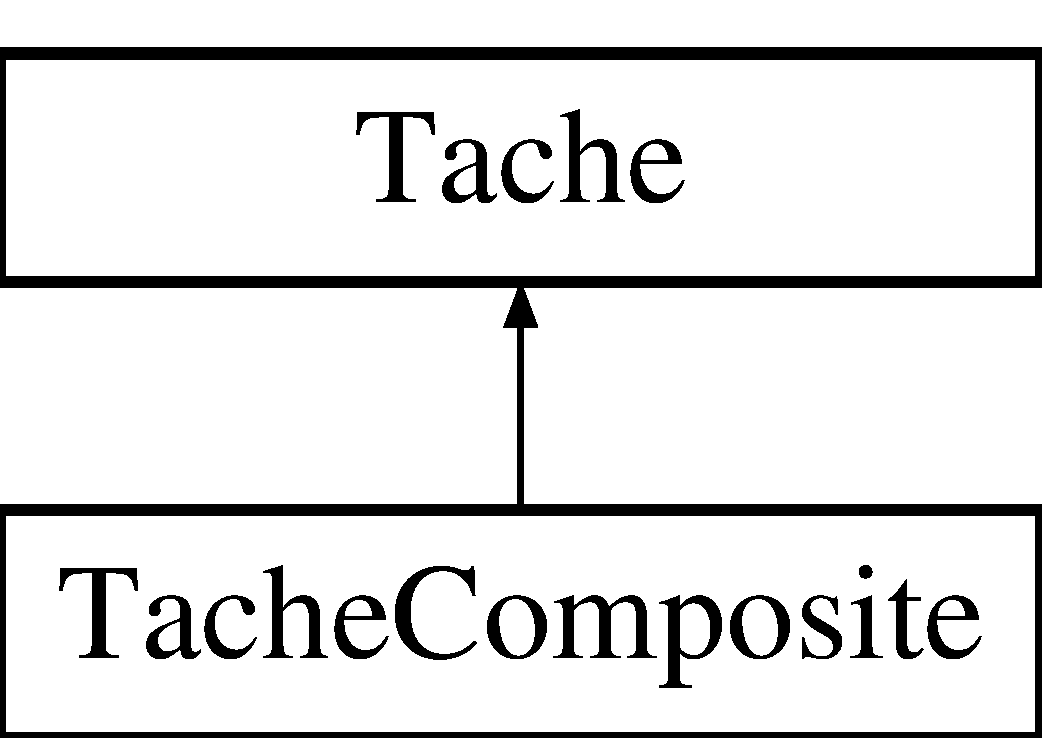
\includegraphics[height=2.000000cm]{class_tache_composite}
\end{center}
\end{figure}
\subsection*{Fonctions membres publiques}
\begin{DoxyCompactItemize}
\item 
void \hyperlink{class_tache_composite_ab4243a926687c17556eeaa34ecbe1567}{add\+Sous\+Tache} (\hyperlink{class_tache}{Tache} $\ast$tache)
\item 
Q\+Vector$<$ \hyperlink{class_tache}{Tache} $\ast$ $>$ \hyperlink{class_tache_composite_a4c7408084fe783835b083501757a1c19}{get\+Liste\+Sous\+Taches} () const 
\end{DoxyCompactItemize}
\subsection*{Fonctions membres privées}
\begin{DoxyCompactItemize}
\item 
\hyperlink{class_tache_composite_a3042d6bf7df70fe0e56f314224fbae53}{Tache\+Composite} (const Q\+String \&id, const Q\+String \&tit, const Q\+String \&desc, \hyperlink{class_projet}{Projet} $\ast$p)
\item 
\hyperlink{class_tache_composite_a073e2621c0bc6cf8e61e2ef6f5e938eb}{Tache\+Composite} (const Q\+String \&id, const Q\+String \&tit, const Q\+String \&desc, const Q\+Date \&dd, const Q\+Date \&de, \hyperlink{class_projet}{Projet} $\ast$p)
\item 
virtual \hyperlink{class_tache_composite_a70ddee42aa910b22a06e8197f5873698}{$\sim$\+Tache\+Composite} ()
\end{DoxyCompactItemize}
\subsection*{Attributs privés}
\begin{DoxyCompactItemize}
\item 
Q\+Vector$<$ \hyperlink{class_tache}{Tache} $\ast$ $>$ \hyperlink{class_tache_composite_ac73545ce9cef80cbdc145a233465df6e}{liste\+Sous\+Taches}
\end{DoxyCompactItemize}
\subsection*{Amis}
\begin{DoxyCompactItemize}
\item 
class \hyperlink{class_tache_composite_ab87b41c3faa36955cc370972f5cce344}{Projet}
\end{DoxyCompactItemize}
\subsection*{Membres hérités additionnels}


\subsection{Documentation des constructeurs et destructeur}
\hypertarget{class_tache_composite_a3042d6bf7df70fe0e56f314224fbae53}{}\index{Tache\+Composite@{Tache\+Composite}!Tache\+Composite@{Tache\+Composite}}
\index{Tache\+Composite@{Tache\+Composite}!Tache\+Composite@{Tache\+Composite}}
\subsubsection[{Tache\+Composite}]{\setlength{\rightskip}{0pt plus 5cm}Tache\+Composite\+::\+Tache\+Composite (
\begin{DoxyParamCaption}
\item[{const Q\+String \&}]{id, }
\item[{const Q\+String \&}]{tit, }
\item[{const Q\+String \&}]{desc, }
\item[{{\bf Projet} $\ast$}]{p}
\end{DoxyParamCaption}
)\hspace{0.3cm}{\ttfamily [private]}}\label{class_tache_composite_a3042d6bf7df70fe0e56f314224fbae53}
\hypertarget{class_tache_composite_a073e2621c0bc6cf8e61e2ef6f5e938eb}{}\index{Tache\+Composite@{Tache\+Composite}!Tache\+Composite@{Tache\+Composite}}
\index{Tache\+Composite@{Tache\+Composite}!Tache\+Composite@{Tache\+Composite}}
\subsubsection[{Tache\+Composite}]{\setlength{\rightskip}{0pt plus 5cm}Tache\+Composite\+::\+Tache\+Composite (
\begin{DoxyParamCaption}
\item[{const Q\+String \&}]{id, }
\item[{const Q\+String \&}]{tit, }
\item[{const Q\+String \&}]{desc, }
\item[{const Q\+Date \&}]{dd, }
\item[{const Q\+Date \&}]{de, }
\item[{{\bf Projet} $\ast$}]{p}
\end{DoxyParamCaption}
)\hspace{0.3cm}{\ttfamily [private]}}\label{class_tache_composite_a073e2621c0bc6cf8e61e2ef6f5e938eb}
\hypertarget{class_tache_composite_a70ddee42aa910b22a06e8197f5873698}{}\index{Tache\+Composite@{Tache\+Composite}!````~Tache\+Composite@{$\sim$\+Tache\+Composite}}
\index{````~Tache\+Composite@{$\sim$\+Tache\+Composite}!Tache\+Composite@{Tache\+Composite}}
\subsubsection[{$\sim$\+Tache\+Composite}]{\setlength{\rightskip}{0pt plus 5cm}Tache\+Composite\+::$\sim$\+Tache\+Composite (
\begin{DoxyParamCaption}
{}
\end{DoxyParamCaption}
)\hspace{0.3cm}{\ttfamily [private]}, {\ttfamily [virtual]}}\label{class_tache_composite_a70ddee42aa910b22a06e8197f5873698}


\subsection{Documentation des fonctions membres}
\hypertarget{class_tache_composite_ab4243a926687c17556eeaa34ecbe1567}{}\index{Tache\+Composite@{Tache\+Composite}!add\+Sous\+Tache@{add\+Sous\+Tache}}
\index{add\+Sous\+Tache@{add\+Sous\+Tache}!Tache\+Composite@{Tache\+Composite}}
\subsubsection[{add\+Sous\+Tache}]{\setlength{\rightskip}{0pt plus 5cm}void Tache\+Composite\+::add\+Sous\+Tache (
\begin{DoxyParamCaption}
\item[{{\bf Tache} $\ast$}]{tache}
\end{DoxyParamCaption}
)}\label{class_tache_composite_ab4243a926687c17556eeaa34ecbe1567}
\hypertarget{class_tache_composite_a4c7408084fe783835b083501757a1c19}{}\index{Tache\+Composite@{Tache\+Composite}!get\+Liste\+Sous\+Taches@{get\+Liste\+Sous\+Taches}}
\index{get\+Liste\+Sous\+Taches@{get\+Liste\+Sous\+Taches}!Tache\+Composite@{Tache\+Composite}}
\subsubsection[{get\+Liste\+Sous\+Taches}]{\setlength{\rightskip}{0pt plus 5cm}Q\+Vector$<${\bf Tache}$\ast$$>$ Tache\+Composite\+::get\+Liste\+Sous\+Taches (
\begin{DoxyParamCaption}
{}
\end{DoxyParamCaption}
) const\hspace{0.3cm}{\ttfamily [inline]}}\label{class_tache_composite_a4c7408084fe783835b083501757a1c19}


\subsection{Documentation des fonctions amies et associées}
\hypertarget{class_tache_composite_ab87b41c3faa36955cc370972f5cce344}{}\index{Tache\+Composite@{Tache\+Composite}!Projet@{Projet}}
\index{Projet@{Projet}!Tache\+Composite@{Tache\+Composite}}
\subsubsection[{Projet}]{\setlength{\rightskip}{0pt plus 5cm}friend class {\bf Projet}\hspace{0.3cm}{\ttfamily [friend]}}\label{class_tache_composite_ab87b41c3faa36955cc370972f5cce344}


\subsection{Documentation des données membres}
\hypertarget{class_tache_composite_ac73545ce9cef80cbdc145a233465df6e}{}\index{Tache\+Composite@{Tache\+Composite}!liste\+Sous\+Taches@{liste\+Sous\+Taches}}
\index{liste\+Sous\+Taches@{liste\+Sous\+Taches}!Tache\+Composite@{Tache\+Composite}}
\subsubsection[{liste\+Sous\+Taches}]{\setlength{\rightskip}{0pt plus 5cm}Q\+Vector$<${\bf Tache}$\ast$$>$ Tache\+Composite\+::liste\+Sous\+Taches\hspace{0.3cm}{\ttfamily [private]}}\label{class_tache_composite_ac73545ce9cef80cbdc145a233465df6e}


La documentation de cette classe a été générée à partir des fichiers suivants \+:\begin{DoxyCompactItemize}
\item 
\hyperlink{tachecomposite_8h}{tachecomposite.\+h}\item 
\hyperlink{tachecomposite_8cpp}{tachecomposite.\+cpp}\end{DoxyCompactItemize}

\hypertarget{class_tache_unitaire}{}\section{Référence de la classe Tache\+Unitaire}
\label{class_tache_unitaire}\index{Tache\+Unitaire@{Tache\+Unitaire}}


{\ttfamily \#include $<$tacheunitaire.\+h$>$}

Graphe d\textquotesingle{}héritage de Tache\+Unitaire\+:\begin{figure}[H]
\begin{center}
\leavevmode
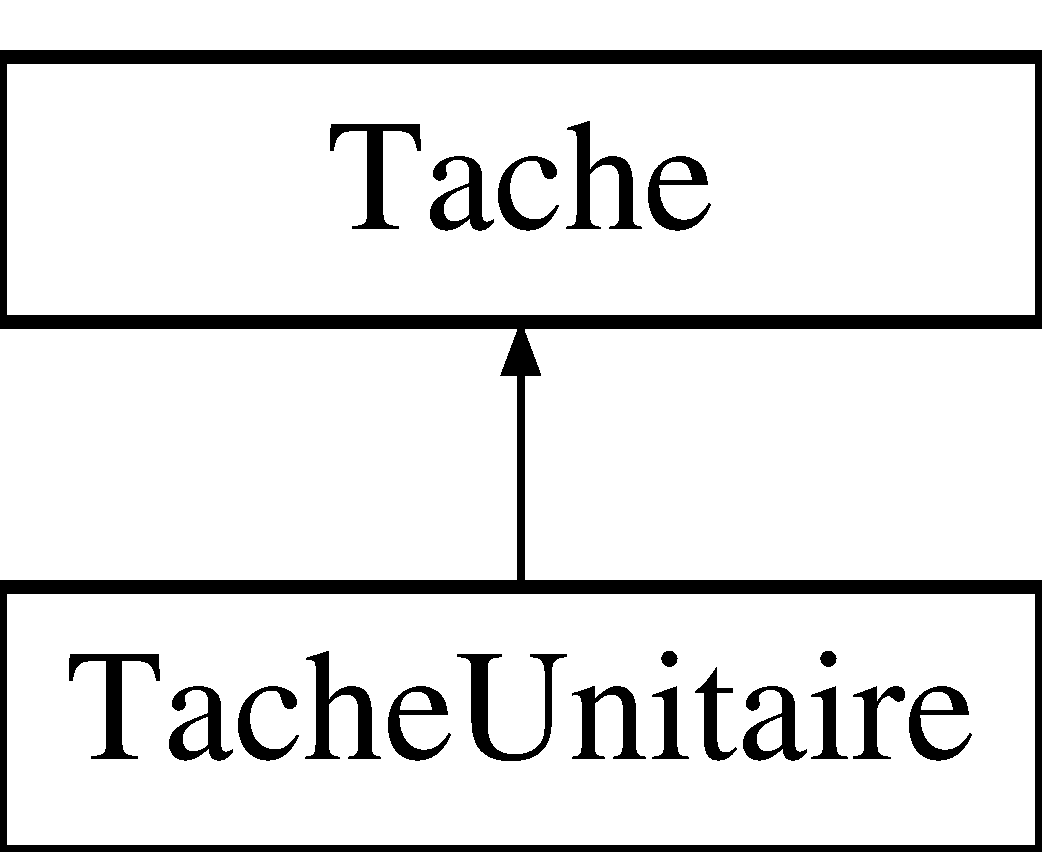
\includegraphics[height=2.000000cm]{class_tache_unitaire}
\end{center}
\end{figure}
\subsection*{Fonctions membres publiques}
\begin{DoxyCompactItemize}
\item 
int \hyperlink{class_tache_unitaire_a2f1c93887c652e5581df4357bc72949b}{get\+Duree} () const 
\item 
int \hyperlink{class_tache_unitaire_aa9b7e58e61dfded16d5a2508d33734c5}{get\+Duree\+Restante} () const 
\item 
void \hyperlink{class_tache_unitaire_a5b1dc4cb5b374fce9c26abb4c954cef8}{set\+Duree\+Restante} (int dur)
\item 
bool \hyperlink{class_tache_unitaire_a4a25bc2f0b3e6ebd6c0617d22328c986}{is\+Preemptee} () const 
\end{DoxyCompactItemize}
\subsection*{Fonctions membres privées}
\begin{DoxyCompactItemize}
\item 
\hyperlink{class_tache_unitaire_acca628b1c239bf191fbbf869ad15cdd2}{Tache\+Unitaire} (const Q\+String \&id, const Q\+String \&tit, const Q\+String \&desc, const int \&dur, const bool \&pre, \hyperlink{class_projet}{Projet} $\ast$p)
\item 
\hyperlink{class_tache_unitaire_ab97fdcb6d8d43ff76d46a7ae650eba3d}{Tache\+Unitaire} (const Q\+String \&id, const Q\+String \&tit, const Q\+String \&desc, const Q\+Date \&dd, const Q\+Date \&de, const int \&dur, const bool \&pre, \hyperlink{class_projet}{Projet} $\ast$p)
\item 
virtual \hyperlink{class_tache_unitaire_a54c9937fb3088c48348883ad1b385f8c}{$\sim$\+Tache\+Unitaire} ()
\end{DoxyCompactItemize}
\subsection*{Attributs privés}
\begin{DoxyCompactItemize}
\item 
int \hyperlink{class_tache_unitaire_a5510c1941069a4391e076ec45e0201fc}{duree}
\item 
int \hyperlink{class_tache_unitaire_a73dd33a7047739e49c80373aeae3158e}{duree\+Restante}
\item 
bool \hyperlink{class_tache_unitaire_a21bc1074f99a80976a52d910e3c21041}{preemptee}
\end{DoxyCompactItemize}
\subsection*{Amis}
\begin{DoxyCompactItemize}
\item 
class \hyperlink{class_tache_unitaire_ab87b41c3faa36955cc370972f5cce344}{Projet}
\end{DoxyCompactItemize}
\subsection*{Membres hérités additionnels}


\subsection{Documentation des constructeurs et destructeur}
\hypertarget{class_tache_unitaire_acca628b1c239bf191fbbf869ad15cdd2}{}\index{Tache\+Unitaire@{Tache\+Unitaire}!Tache\+Unitaire@{Tache\+Unitaire}}
\index{Tache\+Unitaire@{Tache\+Unitaire}!Tache\+Unitaire@{Tache\+Unitaire}}
\subsubsection[{Tache\+Unitaire}]{\setlength{\rightskip}{0pt plus 5cm}Tache\+Unitaire\+::\+Tache\+Unitaire (
\begin{DoxyParamCaption}
\item[{const Q\+String \&}]{id, }
\item[{const Q\+String \&}]{tit, }
\item[{const Q\+String \&}]{desc, }
\item[{const int \&}]{dur, }
\item[{const bool \&}]{pre, }
\item[{{\bf Projet} $\ast$}]{p}
\end{DoxyParamCaption}
)\hspace{0.3cm}{\ttfamily [private]}}\label{class_tache_unitaire_acca628b1c239bf191fbbf869ad15cdd2}
\hypertarget{class_tache_unitaire_ab97fdcb6d8d43ff76d46a7ae650eba3d}{}\index{Tache\+Unitaire@{Tache\+Unitaire}!Tache\+Unitaire@{Tache\+Unitaire}}
\index{Tache\+Unitaire@{Tache\+Unitaire}!Tache\+Unitaire@{Tache\+Unitaire}}
\subsubsection[{Tache\+Unitaire}]{\setlength{\rightskip}{0pt plus 5cm}Tache\+Unitaire\+::\+Tache\+Unitaire (
\begin{DoxyParamCaption}
\item[{const Q\+String \&}]{id, }
\item[{const Q\+String \&}]{tit, }
\item[{const Q\+String \&}]{desc, }
\item[{const Q\+Date \&}]{dd, }
\item[{const Q\+Date \&}]{de, }
\item[{const int \&}]{dur, }
\item[{const bool \&}]{pre, }
\item[{{\bf Projet} $\ast$}]{p}
\end{DoxyParamCaption}
)\hspace{0.3cm}{\ttfamily [private]}}\label{class_tache_unitaire_ab97fdcb6d8d43ff76d46a7ae650eba3d}
\hypertarget{class_tache_unitaire_a54c9937fb3088c48348883ad1b385f8c}{}\index{Tache\+Unitaire@{Tache\+Unitaire}!````~Tache\+Unitaire@{$\sim$\+Tache\+Unitaire}}
\index{````~Tache\+Unitaire@{$\sim$\+Tache\+Unitaire}!Tache\+Unitaire@{Tache\+Unitaire}}
\subsubsection[{$\sim$\+Tache\+Unitaire}]{\setlength{\rightskip}{0pt plus 5cm}Tache\+Unitaire\+::$\sim$\+Tache\+Unitaire (
\begin{DoxyParamCaption}
{}
\end{DoxyParamCaption}
)\hspace{0.3cm}{\ttfamily [private]}, {\ttfamily [virtual]}}\label{class_tache_unitaire_a54c9937fb3088c48348883ad1b385f8c}


\subsection{Documentation des fonctions membres}
\hypertarget{class_tache_unitaire_a2f1c93887c652e5581df4357bc72949b}{}\index{Tache\+Unitaire@{Tache\+Unitaire}!get\+Duree@{get\+Duree}}
\index{get\+Duree@{get\+Duree}!Tache\+Unitaire@{Tache\+Unitaire}}
\subsubsection[{get\+Duree}]{\setlength{\rightskip}{0pt plus 5cm}int Tache\+Unitaire\+::get\+Duree (
\begin{DoxyParamCaption}
{}
\end{DoxyParamCaption}
) const\hspace{0.3cm}{\ttfamily [inline]}}\label{class_tache_unitaire_a2f1c93887c652e5581df4357bc72949b}
\hypertarget{class_tache_unitaire_aa9b7e58e61dfded16d5a2508d33734c5}{}\index{Tache\+Unitaire@{Tache\+Unitaire}!get\+Duree\+Restante@{get\+Duree\+Restante}}
\index{get\+Duree\+Restante@{get\+Duree\+Restante}!Tache\+Unitaire@{Tache\+Unitaire}}
\subsubsection[{get\+Duree\+Restante}]{\setlength{\rightskip}{0pt plus 5cm}int Tache\+Unitaire\+::get\+Duree\+Restante (
\begin{DoxyParamCaption}
{}
\end{DoxyParamCaption}
) const\hspace{0.3cm}{\ttfamily [inline]}}\label{class_tache_unitaire_aa9b7e58e61dfded16d5a2508d33734c5}
\hypertarget{class_tache_unitaire_a4a25bc2f0b3e6ebd6c0617d22328c986}{}\index{Tache\+Unitaire@{Tache\+Unitaire}!is\+Preemptee@{is\+Preemptee}}
\index{is\+Preemptee@{is\+Preemptee}!Tache\+Unitaire@{Tache\+Unitaire}}
\subsubsection[{is\+Preemptee}]{\setlength{\rightskip}{0pt plus 5cm}bool Tache\+Unitaire\+::is\+Preemptee (
\begin{DoxyParamCaption}
{}
\end{DoxyParamCaption}
) const\hspace{0.3cm}{\ttfamily [inline]}}\label{class_tache_unitaire_a4a25bc2f0b3e6ebd6c0617d22328c986}
\hypertarget{class_tache_unitaire_a5b1dc4cb5b374fce9c26abb4c954cef8}{}\index{Tache\+Unitaire@{Tache\+Unitaire}!set\+Duree\+Restante@{set\+Duree\+Restante}}
\index{set\+Duree\+Restante@{set\+Duree\+Restante}!Tache\+Unitaire@{Tache\+Unitaire}}
\subsubsection[{set\+Duree\+Restante}]{\setlength{\rightskip}{0pt plus 5cm}void Tache\+Unitaire\+::set\+Duree\+Restante (
\begin{DoxyParamCaption}
\item[{int}]{dur}
\end{DoxyParamCaption}
)\hspace{0.3cm}{\ttfamily [inline]}}\label{class_tache_unitaire_a5b1dc4cb5b374fce9c26abb4c954cef8}


\subsection{Documentation des fonctions amies et associées}
\hypertarget{class_tache_unitaire_ab87b41c3faa36955cc370972f5cce344}{}\index{Tache\+Unitaire@{Tache\+Unitaire}!Projet@{Projet}}
\index{Projet@{Projet}!Tache\+Unitaire@{Tache\+Unitaire}}
\subsubsection[{Projet}]{\setlength{\rightskip}{0pt plus 5cm}friend class {\bf Projet}\hspace{0.3cm}{\ttfamily [friend]}}\label{class_tache_unitaire_ab87b41c3faa36955cc370972f5cce344}


\subsection{Documentation des données membres}
\hypertarget{class_tache_unitaire_a5510c1941069a4391e076ec45e0201fc}{}\index{Tache\+Unitaire@{Tache\+Unitaire}!duree@{duree}}
\index{duree@{duree}!Tache\+Unitaire@{Tache\+Unitaire}}
\subsubsection[{duree}]{\setlength{\rightskip}{0pt plus 5cm}int Tache\+Unitaire\+::duree\hspace{0.3cm}{\ttfamily [private]}}\label{class_tache_unitaire_a5510c1941069a4391e076ec45e0201fc}
\hypertarget{class_tache_unitaire_a73dd33a7047739e49c80373aeae3158e}{}\index{Tache\+Unitaire@{Tache\+Unitaire}!duree\+Restante@{duree\+Restante}}
\index{duree\+Restante@{duree\+Restante}!Tache\+Unitaire@{Tache\+Unitaire}}
\subsubsection[{duree\+Restante}]{\setlength{\rightskip}{0pt plus 5cm}int Tache\+Unitaire\+::duree\+Restante\hspace{0.3cm}{\ttfamily [private]}}\label{class_tache_unitaire_a73dd33a7047739e49c80373aeae3158e}
\hypertarget{class_tache_unitaire_a21bc1074f99a80976a52d910e3c21041}{}\index{Tache\+Unitaire@{Tache\+Unitaire}!preemptee@{preemptee}}
\index{preemptee@{preemptee}!Tache\+Unitaire@{Tache\+Unitaire}}
\subsubsection[{preemptee}]{\setlength{\rightskip}{0pt plus 5cm}bool Tache\+Unitaire\+::preemptee\hspace{0.3cm}{\ttfamily [private]}}\label{class_tache_unitaire_a21bc1074f99a80976a52d910e3c21041}


La documentation de cette classe a été générée à partir des fichiers suivants \+:\begin{DoxyCompactItemize}
\item 
\hyperlink{tacheunitaire_8h}{tacheunitaire.\+h}\item 
\hyperlink{tacheunitaire_8cpp}{tacheunitaire.\+cpp}\end{DoxyCompactItemize}

\chapter{Documentation des fichiers}
\hypertarget{interface_8cpp}{}\section{Référence du fichier interface.\+cpp}
\label{interface_8cpp}\index{interface.\+cpp@{interface.\+cpp}}
{\ttfamily \#include \char`\"{}Interface.\+h\char`\"{}}\\*

\hypertarget{interface_8h}{}\section{Référence du fichier interface.\+h}
\label{interface_8h}\index{interface.\+h@{interface.\+h}}
{\ttfamily \#include $<$iostream$>$}\\*
{\ttfamily \#include $<$Q\+List$>$}\\*
{\ttfamily \#include $<$Q\+Object$>$}\\*
{\ttfamily \#include $<$Q\+Widget$>$}\\*
{\ttfamily \#include $<$Q\+Main\+Window$>$}\\*
{\ttfamily \#include $<$Q\+Menu\+Bar$>$}\\*
{\ttfamily \#include $<$Q\+Menu$>$}\\*
{\ttfamily \#include $<$Q\+String$>$}\\*
{\ttfamily \#include $<$Q\+Label$>$}\\*
{\ttfamily \#include $<$Q\+V\+Box\+Layout$>$}\\*
{\ttfamily \#include $<$Q\+H\+Box\+Layout$>$}\\*
{\ttfamily \#include $<$Q\+Table\+Widget$>$}\\*
{\ttfamily \#include $<$Q\+String\+List$>$}\\*
{\ttfamily \#include $<$Q\+Date\+Edit$>$}\\*
{\ttfamily \#include $<$Q\+Date$>$}\\*
{\ttfamily \#include $<$Q\+Action$>$}\\*
{\ttfamily \#include $<$Q\+File\+Dialog$>$}\\*
{\ttfamily \#include $<$Q\+Message\+Box$>$}\\*
{\ttfamily \#include $<$Q\+Brush$>$}\\*
{\ttfamily \#include $<$Q\+Color$>$}\\*
{\ttfamily \#include $<$Q\+Calendar\+Widget$>$}\\*
{\ttfamily \#include $<$Q\+Header\+View$>$}\\*
{\ttfamily \#include $<$Q\+Group\+Box$>$}\\*
{\ttfamily \#include $<$Q\+Push\+Button$>$}\\*
\subsection*{Classes}
\begin{DoxyCompactItemize}
\item 
class \hyperlink{class_interface}{Interface}
\end{DoxyCompactItemize}

\hypertarget{listeprojets_8cpp}{}\section{projet/listeprojets.cpp File Reference}
\label{listeprojets_8cpp}\index{projet/listeprojets.\+cpp@{projet/listeprojets.\+cpp}}
{\ttfamily \#include \char`\"{}listeprojets.\+h\char`\"{}}\\*
{\ttfamily \#include \char`\"{}afficheprojet.\+h\char`\"{}}\\*
{\ttfamily \#include \char`\"{}ajouteprojet.\+h\char`\"{}}\\*

\hypertarget{listeprojets_8h}{}\section{Référence du fichier listeprojets.\+h}
\label{listeprojets_8h}\index{listeprojets.\+h@{listeprojets.\+h}}
{\ttfamily \#include $<$Q\+Object$>$}\\*
{\ttfamily \#include $<$Q\+Widget$>$}\\*
{\ttfamily \#include $<$Q\+Dialog$>$}\\*
\subsection*{Classes}
\begin{DoxyCompactItemize}
\item 
class \hyperlink{class_liste_projets}{Liste\+Projets}
\end{DoxyCompactItemize}

\hypertarget{main_8cpp}{}\section{Référence du fichier main.\+cpp}
\label{main_8cpp}\index{main.\+cpp@{main.\+cpp}}
{\ttfamily \#include \char`\"{}mainwindow.\+h\char`\"{}}\\*
{\ttfamily \#include $<$Q\+Application$>$}\\*
{\ttfamily \#include $<$iostream$>$}\\*
{\ttfamily \#include $<$Q\+String$>$}\\*
{\ttfamily \#include $<$q\+Debug$>$}\\*
{\ttfamily \#include \char`\"{}tache.\+h\char`\"{}}\\*
{\ttfamily \#include \char`\"{}projet.\+h\char`\"{}}\\*
{\ttfamily \#include \char`\"{}projetmanager.\+h\char`\"{}}\\*
{\ttfamily \#include \char`\"{}programmationmanager.\+h\char`\"{}}\\*
{\ttfamily \#include \char`\"{}interface.\+h\char`\"{}}\\*
{\ttfamily \#include \char`\"{}listeprojets.\+h\char`\"{}}\\*
\subsection*{Fonctions}
\begin{DoxyCompactItemize}
\item 
int \hyperlink{main_8cpp_a0ddf1224851353fc92bfbff6f499fa97}{main} (int argc, char $\ast$argv\mbox{[}$\,$\mbox{]})
\end{DoxyCompactItemize}


\subsection{Documentation des fonctions}
\hypertarget{main_8cpp_a0ddf1224851353fc92bfbff6f499fa97}{}\index{main.\+cpp@{main.\+cpp}!main@{main}}
\index{main@{main}!main.\+cpp@{main.\+cpp}}
\subsubsection[{main}]{\setlength{\rightskip}{0pt plus 5cm}int main (
\begin{DoxyParamCaption}
\item[{int}]{argc, }
\item[{char $\ast$}]{argv\mbox{[}$\,$\mbox{]}}
\end{DoxyParamCaption}
)}\label{main_8cpp_a0ddf1224851353fc92bfbff6f499fa97}

\hypertarget{mainwindow_8cpp}{}\section{projet/mainwindow.cpp File Reference}
\label{mainwindow_8cpp}\index{projet/mainwindow.\+cpp@{projet/mainwindow.\+cpp}}
{\ttfamily \#include \char`\"{}mainwindow.\+h\char`\"{}}\\*
{\ttfamily \#include \char`\"{}ui\+\_\+mainwindow.\+h\char`\"{}}\\*

\hypertarget{mainwindow_8h}{}\section{projet/mainwindow.h File Reference}
\label{mainwindow_8h}\index{projet/mainwindow.\+h@{projet/mainwindow.\+h}}
{\ttfamily \#include $<$Q\+Main\+Window$>$}\\*
\subsection*{Classes}
\begin{DoxyCompactItemize}
\item 
class \hyperlink{class_main_window}{Main\+Window}
\end{DoxyCompactItemize}
\subsection*{Namespaces}
\begin{DoxyCompactItemize}
\item 
 \hyperlink{namespace_ui}{Ui}
\end{DoxyCompactItemize}

\hypertarget{programmation_8cpp}{}\section{projet/programmation.cpp File Reference}
\label{programmation_8cpp}\index{projet/programmation.\+cpp@{projet/programmation.\+cpp}}
{\ttfamily \#include $<$Q\+Debug$>$}\\*
{\ttfamily \#include \char`\"{}programmation.\+h\char`\"{}}\\*

\hypertarget{programmation_8h}{}\section{projet/programmation.h File Reference}
\label{programmation_8h}\index{projet/programmation.\+h@{projet/programmation.\+h}}
{\ttfamily \#include $<$Q\+Date$>$}\\*
{\ttfamily \#include $<$Q\+String$>$}\\*
{\ttfamily \#include \char`\"{}tache.\+h\char`\"{}}\\*
\subsection*{Classes}
\begin{DoxyCompactItemize}
\item 
class \hyperlink{class_programmation}{Programmation}
\begin{DoxyCompactList}\small\item\em Classe représentant une \hyperlink{class_programmation}{Programmation}. \end{DoxyCompactList}\end{DoxyCompactItemize}

\hypertarget{programmationactivite_8cpp}{}\section{projet/programmationactivite.cpp File Reference}
\label{programmationactivite_8cpp}\index{projet/programmationactivite.\+cpp@{projet/programmationactivite.\+cpp}}
{\ttfamily \#include $<$Q\+Debug$>$}\\*
{\ttfamily \#include \char`\"{}programmationactivite.\+h\char`\"{}}\\*

\hypertarget{programmationactivite_8h}{}\section{Référence du fichier programmationactivite.\+h}
\label{programmationactivite_8h}\index{programmationactivite.\+h@{programmationactivite.\+h}}
{\ttfamily \#include \char`\"{}programmation.\+h\char`\"{}}\\*
\subsection*{Classes}
\begin{DoxyCompactItemize}
\item 
class \hyperlink{class_programmation_activite}{Programmation\+Activite}
\end{DoxyCompactItemize}

\hypertarget{programmationmanager_8cpp}{}\section{Référence du fichier programmationmanager.\+cpp}
\label{programmationmanager_8cpp}\index{programmationmanager.\+cpp@{programmationmanager.\+cpp}}
{\ttfamily \#include $<$Q\+Debug$>$}\\*
{\ttfamily \#include \char`\"{}Tache\+Unitaire.\+h\char`\"{}}\\*
{\ttfamily \#include \char`\"{}Programmation\+Manager.\+h\char`\"{}}\\*

\hypertarget{programmationmanager_8h}{}\section{projet/programmationmanager.h File Reference}
\label{programmationmanager_8h}\index{projet/programmationmanager.\+h@{projet/programmationmanager.\+h}}
{\ttfamily \#include $<$Q\+Vector$>$}\\*
{\ttfamily \#include \char`\"{}programmation.\+h\char`\"{}}\\*
{\ttfamily \#include \char`\"{}programmationtache.\+h\char`\"{}}\\*
{\ttfamily \#include \char`\"{}programmationactivite.\+h\char`\"{}}\\*
\subsection*{Classes}
\begin{DoxyCompactItemize}
\item 
class \hyperlink{class_programmation_manager}{Programmation\+Manager}
\begin{DoxyCompactList}\small\item\em Classe représentant le manager de \hyperlink{class_programmation}{Programmation}. \end{DoxyCompactList}\end{DoxyCompactItemize}

\hypertarget{programmationtache_8cpp}{}\section{Référence du fichier programmationtache.\+cpp}
\label{programmationtache_8cpp}\index{programmationtache.\+cpp@{programmationtache.\+cpp}}
{\ttfamily \#include $<$Q\+Debug$>$}\\*
{\ttfamily \#include \char`\"{}Programmation\+Tache.\+h\char`\"{}}\\*

\hypertarget{programmationtache_8h}{}\section{projet/programmationtache.h File Reference}
\label{programmationtache_8h}\index{projet/programmationtache.\+h@{projet/programmationtache.\+h}}
{\ttfamily \#include \char`\"{}programmation.\+h\char`\"{}}\\*
\subsection*{Classes}
\begin{DoxyCompactItemize}
\item 
class \hyperlink{class_programmation_tache}{Programmation\+Tache}
\begin{DoxyCompactList}\small\item\em Classe représentant une \hyperlink{class_programmation_tache}{Programmation\+Tache}. \end{DoxyCompactList}\end{DoxyCompactItemize}

\hypertarget{projet_8cpp}{}\section{Référence du fichier projet.\+cpp}
\label{projet_8cpp}\index{projet.\+cpp@{projet.\+cpp}}
{\ttfamily \#include $<$Q\+Debug$>$}\\*
{\ttfamily \#include $<$Q\+Vector$>$}\\*
{\ttfamily \#include $<$Q\+Date$>$}\\*
{\ttfamily \#include \char`\"{}projet.\+h\char`\"{}}\\*
{\ttfamily \#include \char`\"{}tache.\+h\char`\"{}}\\*

\hypertarget{projet_8h}{}\section{projet/projet.h File Reference}
\label{projet_8h}\index{projet/projet.\+h@{projet/projet.\+h}}
{\ttfamily \#include $<$Q\+Vector$>$}\\*
{\ttfamily \#include $<$Q\+Date$>$}\\*
{\ttfamily \#include \char`\"{}tache.\+h\char`\"{}}\\*
{\ttfamily \#include \char`\"{}tacheunitaire.\+h\char`\"{}}\\*
{\ttfamily \#include \char`\"{}tachecomposite.\+h\char`\"{}}\\*
\subsection*{Classes}
\begin{DoxyCompactItemize}
\item 
class \hyperlink{class_projet}{Projet}
\begin{DoxyCompactList}\small\item\em Classe représentant un \hyperlink{class_projet}{Projet}. \end{DoxyCompactList}\end{DoxyCompactItemize}

\hypertarget{projetmanager_8cpp}{}\section{projet/projetmanager.cpp File Reference}
\label{projetmanager_8cpp}\index{projet/projetmanager.\+cpp@{projet/projetmanager.\+cpp}}
{\ttfamily \#include $<$Q\+Debug$>$}\\*
{\ttfamily \#include \char`\"{}projetmanager.\+h\char`\"{}}\\*
{\ttfamily \#include \char`\"{}projet.\+h\char`\"{}}\\*

\hypertarget{projetmanager_8h}{}\section{projet/projetmanager.h File Reference}
\label{projetmanager_8h}\index{projet/projetmanager.\+h@{projet/projetmanager.\+h}}
{\ttfamily \#include $<$Q\+Vector$>$}\\*
{\ttfamily \#include \char`\"{}Projet.\+h\char`\"{}}\\*
\subsection*{Classes}
\begin{DoxyCompactItemize}
\item 
class \hyperlink{class_projet_manager}{Projet\+Manager}
\begin{DoxyCompactList}\small\item\em Classe représentant le manager de \hyperlink{class_projet}{Projet}. \end{DoxyCompactList}\end{DoxyCompactItemize}

\hypertarget{tache_8cpp}{}\section{Référence du fichier tache.\+cpp}
\label{tache_8cpp}\index{tache.\+cpp@{tache.\+cpp}}
{\ttfamily \#include $<$Q\+Debug$>$}\\*
{\ttfamily \#include $<$iostream$>$}\\*
{\ttfamily \#include \char`\"{}tache.\+h\char`\"{}}\\*
{\ttfamily \#include \char`\"{}projet.\+h\char`\"{}}\\*
{\ttfamily \#include \char`\"{}tachecomposite.\+h\char`\"{}}\\*

\hypertarget{tache_8h}{}\section{projet/tache.h File Reference}
\label{tache_8h}\index{projet/tache.\+h@{projet/tache.\+h}}
{\ttfamily \#include $<$Q\+Date$>$}\\*
{\ttfamily \#include $<$Q\+String$>$}\\*
{\ttfamily \#include $<$Q\+Vector$>$}\\*
\subsection*{Classes}
\begin{DoxyCompactItemize}
\item 
class \hyperlink{class_tache}{Tache}
\begin{DoxyCompactList}\small\item\em Classe représentant une tâche. \end{DoxyCompactList}\end{DoxyCompactItemize}

\hypertarget{tachecomposite_8cpp}{}\section{Référence du fichier tachecomposite.\+cpp}
\label{tachecomposite_8cpp}\index{tachecomposite.\+cpp@{tachecomposite.\+cpp}}
{\ttfamily \#include $<$Q\+Debug$>$}\\*
{\ttfamily \#include \char`\"{}tachecomposite.\+h\char`\"{}}\\*

\hypertarget{tachecomposite_8h}{}\section{projet/tachecomposite.h File Reference}
\label{tachecomposite_8h}\index{projet/tachecomposite.\+h@{projet/tachecomposite.\+h}}
{\ttfamily \#include \char`\"{}tache.\+h\char`\"{}}\\*
\subsection*{Classes}
\begin{DoxyCompactItemize}
\item 
class \hyperlink{class_tache_composite}{Tache\+Composite}
\begin{DoxyCompactList}\small\item\em Classe représentant une \hyperlink{class_tache_composite}{Tache\+Composite}. \end{DoxyCompactList}\end{DoxyCompactItemize}

\hypertarget{tacheunitaire_8cpp}{}\section{Référence du fichier tacheunitaire.\+cpp}
\label{tacheunitaire_8cpp}\index{tacheunitaire.\+cpp@{tacheunitaire.\+cpp}}
{\ttfamily \#include $<$Q\+Debug$>$}\\*
{\ttfamily \#include \char`\"{}tacheunitaire.\+h\char`\"{}}\\*

\hypertarget{tacheunitaire_8h}{}\section{Référence du fichier tacheunitaire.\+h}
\label{tacheunitaire_8h}\index{tacheunitaire.\+h@{tacheunitaire.\+h}}
{\ttfamily \#include \char`\"{}tache.\+h\char`\"{}}\\*
\subsection*{Classes}
\begin{DoxyCompactItemize}
\item 
class \hyperlink{class_tache_unitaire}{Tache\+Unitaire}
\end{DoxyCompactItemize}

%--- End generated contents ---

% Index
\backmatter
\newpage
\phantomsection
\clearemptydoublepage
\addcontentsline{toc}{chapter}{Index}
\printindex

\end{document}
